%=================================================================
% Fractal and Fractional (MDPI) submission
% Spectral Isomorphism ... Non-Autonomous Quadratic Maps and Riemann Zeros
%=================================================================
\documentclass[mca,article,submit,oneauthor,pdftex]{Definitions/mdpi}

\firstpage{1}
\makeatletter
\setcounter{page}{\@firstpage}
\makeatother
\pubvolume{1}
\issuenum{1}
\articlenumber{0}
\pubyear{2026}
\copyrightyear{2026}
\datereceived{ }
\daterevised{ }
\dateaccepted{ }
\datepublished{ }

% extra packages (most already loaded by the class)
\usepackage{longtable,booktabs,array,tabularx}
\newcolumntype{Y}[1]{>{\hsize=#1\hsize\raggedright\arraybackslash}X}
\providecommand{\tightlist}{\setlength{\itemsep}{0pt}\setlength{\parskip}{0pt}}

%=================================================================
\Title{Numerical Spectral Correspondence between a Non-Autonomous Quadratic Map and the Riemann Zeros: An Exploratory Study}

%\newcommand{\orcidauthorA}{0000-0000-0000-0000}

\Author{Liang Wang}

\AuthorNames{Liang Wang}

\address[1]{%
School of Artificial Intelligence and Automation, Huazhong University of Science and Technology, Wuhan 430070, P.R. China; wangliang.f@gmail.com}

\corres{Correspondence: wangliang.f@gmail.com}

\abstract{This study examines a non-autonomous quadratic map driven by a logarithmic cooling schedule ($\mu_n \sim 1/\ln^2 n$, a phenomenological ansatz), building on the author's recent result that the logistic map's symbolic dynamics at its band-merging point is isomorphic to the prime sieve \cite{wang2026}. From its trajectories the author constructs an empirical, non-normal, dissipative transfer matrix and compares its complex eigenphases to the non-trivial Riemann zeros after calibrating a few free parameters against the same low-order zeros -- an in-sample numerical correspondence, not an independent prediction. The author quantifies this gap directly: fitting on the first $M\in\{50,70,80\}$ zeros and evaluating on the rest gives a held-out MSE one to two orders of magnitude larger than the training error, with the fitted coupling drifting across $M$ but remaining comparatively stable across ten random seeds at fixed $M=70$ (CV $\approx4.7\%$). At low order ($N\lesssim 20$), an unselected re-computation shows a qualitative rank correlation ($\rho=0.56$, $p=0.010$) with, but no significant joint co-location ($p=0.099$) of, a residual feature reported in recent ion-trap quantum simulations of the same zeros. At larger $N$ ($N\ge 1000$), the model matches a globally rescaled GUE surrogate's mean counting-function trend better once conjugate eigenphases are restored, though this partly follows from the construction's own symmetry; a separate, standard unfolded local-statistics test shows the model's own eigenphase spacings do \emph{not} match GUE, unlike the true zeros. These are numerical observations on a heuristic model, not a proof or Hilbert--P\'olya-type operator construction; Table~\ref{tab:claims} tabulates the epistemic status of every main claim.}

\keyword{Riemann zeros; non-autonomous dynamical systems; logistic map; transfer operator; empirical spectral correspondence; numerical continuation}

\MSC{11M26; 37E05; 65P20}

\begin{document}

\maketitle

\section{Introduction}

Since the seminal hypothesis by Riemann \cite{riemann1859}, finding a Hermitian
operator whose eigenvalues correspond to the imaginary parts of
the non-trivial Riemann zeros has always been the ``central open problem'' in the
field of mathematical physics (i.e., the famous Hilbert-P\'olya
conjecture; see \cite{katzsarnak1999,schumayer2011,conrey2003} for reviews),
and the search for a concrete such operator remains active, e.g.\ the
recent explicit Hamiltonian construction of Yakaboylu \cite{yakaboylu2024}.
The zeros themselves are inseparable from the classical theory of prime
counting: their existence and analytic continuation underlie the Prime
Number Theorem, independently established by Hadamard \cite{hadamard1896} and
de la Vall\'ee Poussin \cite{delavallee1896}, and their finer statistics touch
on the Hardy--Littlewood conjectures for prime constellations
\cite{hardylittlewood1923}. The classical analytic theory of \(\zeta(s)\)
itself is treated comprehensively in Titchmarsh's monograph
\cite{titchmarsh1951}, and large-scale numerical verification of the
zeros' locations was pioneered by Odlyzko \cite{odlyzko1989}, with such
high-precision numerical evaluation of $\zeta(s)$ still an active line of
methodological work today \cite{orellana2025}. Over half a
century after Riemann, the pioneering work of
Montgomery \cite{montgomery1973} and numerical verifications by Odlyzko \cite{odlyzko1987}
established a notable connection between the Riemann zero spacing and
the Gaussian Unitary Ensemble (GUE) of Random Matrix Theory (RMT), whose
statistical machinery traces back to Wigner's semicircle law for nuclear
energy levels \cite{wigner1955} and was later codified in Mehta's
treatise \cite{mehta2004}. This spacing statistics connection was
subsequently generalized by Katz and Sarnak to families of \(L\)-functions
\cite{katzsarnak1999,rudnicksarnak1996} and refined through the moments
conjecture of Keating and Snaith \cite{keatingsnaith2000}, connecting
this number-theoretic problem to the physics of Quantum Chaos
\cite{berry1986}. On the physics side, the semiclassical link between
chaotic spectra and RMT statistics is the content of the
Bohigas--Giannoni--Schmit conjecture \cite{bohigas1984}, itself grounded in
Gutzwiller's periodic-orbit trace formula \cite{gutzwiller1971} and its
number-theoretic analogue, the Selberg trace formula \cite{selberg1956}; by
contrast, generic integrable systems display Poissonian level statistics
\cite{berrytabor1977}. Subsequently, Sir Michael Berry and
Keating proposed the renowned \(\text{H}\text{=}\text{xp}\) quantum
Hamiltonian conjecture \cite{berry1999}, later developed by Sierra and
collaborators into explicit spectral realizations of the Riemann zeros
\cite{sierra2009,sierrarodriguez2011}. Other models, such as those based on
non-commutative geometry \cite{connes1999}, have also been explored. However,
existing analytical models generally derive the
macroscopic statistical laws (GUE distribution) of high-order zeros well, but
rarely generate the specific, discrete
coordinates of low-order zeros deterministically from first principles.
Constructing a deterministic dynamical system that reproduces the
true Riemann spectrum from first principles remains an open problem.

In recent years, with advances in quantum information technology,
physicists have begun attempting to ``physically'' find Riemann zeros in
the laboratory \cite{he2020}. For example, a team from the University of Science and
Technology of China (USTC) measured the first 80 Riemann
zeros on physical equipment using Floquet engineering by periodically
driving qubits in an Ion Trap with microwaves \cite{he2021}. Although the
low-frequency band achieved high fidelity, the experiment
simultaneously reported an unexplained feature: when approaching
specific energy levels (e.g., \(\text{N} \text{\ensuremath{\approx} 20}\)), the measurement
deviation of the physical instruments showed a large divergence
(enlarged error bars) that departed from a conventional Gaussian background.
Floquet-engineered simulation of driven quantum systems has itself continued
to scale on near-term hardware since then \cite{eckstein2024}, underscoring
that the platform is an active target for larger-scale zero-finding
experiments rather than a one-off demonstration. The physics community still lacks a unified theoretical framework to
explain this: whether it is due purely to instrumental engineering
decoherence such as laser linewidth, or in part to some intrinsic limit
encountered by the system when approximating highly nonlinear
manifolds remains an open question the author does not resolve here---a question
that touches upon the fundamental asymptotics of
eigenvalue distribution originally discussed by Weyl \cite{weyl1912}.

Rather than starting from an analytically motivated Hamiltonian, the author takes an
exploratory, ``bottom-up'' route, motivated by the author's recent finding that the
symbolic dynamics of the Logistic map at its band-merging point is
isomorphic to the prime sieve, with the Hardy--Littlewood twin-prime
constant emerging as a fixed point of the dynamics \cite{wang2026}. Since
that work connects a deterministic map to the arithmetic of the primes, it
is natural to ask, purely as a numerical experiment, what the eigenphase
spectrum of an empirical transfer operator built from a related map looks
like, and whether it bears any quantitative resemblance to the Riemann
zeros; the author emphasizes at the outset that this question, and everything that
follows from it, is explored numerically and heuristically, and that the author does
not construct or claim to approximate a self-adjoint Hilbert--P\'olya
operator. The approach taken here also
draws on the classical observations that simple maps can have complicated
dynamics \cite{may1976,liyorke1975} and on the universality of nonlinear transformations
\cite{feigenbaum1978}, independently derived via renormalization-group
iteration by Coullet and Tresser \cite{coullettresser1978} and
systematized in the reprint collection of Cvitanovi\'c
\cite{cvitanovic1984}; the underlying combinatorial structure of the
period-doubling cascade itself was first classified by Metropolis, Stein
and Stein \cite{metropolis1973}. Concretely, the author discards the autonomous static potential
and constructs a discrete Markov evolution operator with non-autonomous
(time-dependent) parameter, in the spirit of Ulam and von Neumann's original
proposal to approximate deterministic chaotic maps by finite Markov chains
\cite{ulam1947,ulam1960}, whose ergodic-theoretic justification (existence of
absolutely continuous invariant measures for piecewise-monotonic maps) is due
to Lasota and Yorke \cite{lasotayorke1973}; broader treatments of quantum
chaos and its RMT signatures appear in \cite{gutzwiller1990,casati1995}. Using large-scale parallel computation and
Arnoldi iteration \cite{arpack1998}, the author searches at high resolution
(\(\text{\ensuremath{\epsilon}\ensuremath{\approx}}\text{10}^{\text{\ensuremath{-}3}}\)) for dynamical trajectories that
trigger a sharp numerical convergence transition in the system.

Next, the author presents the non-autonomous dynamical model. The author reports numerical
correspondences between an empirical transfer-matrix spectrum and the
Riemann zeros across scales, from low-order eigenphase alignment (obtained
after calibrating a small number of free parameters against the same
low-order zeros) to macroscopic asymptotic behavior. The author then examine the
model's dependence on numerical resolution and discuss how breaking the
intrinsic conjugate symmetry of the eigenphase spectrum (a consequence of
$P$ being a real-valued matrix) affects the
macroscopic fit. Table~\ref{tab:claims} in the Discussion states the
epistemic status of each claim explicitly.

\section{The Mathematical Model}\label{sec:model}

\subsection{The Dynamic Kernel: Non-autonomous Logistic Map}

The present work considers a classical, deterministic non-autonomous dynamical system on
the interval \(\text{[\ensuremath{-}1, 1]}\); no Hilbert-space operator or
unitary evolution is postulated or constructed at any point in this work.
The microscopic evolution is
governed by the canonical Non-autonomous Quadratic Map (topologically
conjugate to the Logistic Map):

\begin{equation}\label{eq:map}
x_{n+1} = 1 - \lambda_n\, x_n^{2},
\end{equation}

In standard chaos theory, the control parameter \(\text{\ensuremath{\lambda}}\) is
typically a constant (e.g., the Feigenbaum accumulation point
\(\text{\ensuremath{\lambda}}_{\text{\ensuremath{\infty}}}\text{\ensuremath{\approx}1.401}\)). However, to match the logarithmic
density distribution of Riemann zeros (Weyl's Law), the author must break the
system's time-translation symmetry. The author introduces an explicit
non-autonomous drive mechanism where the control parameter
\(\text{\ensuremath{\lambda}}_{\text{n}}\) evolves with the iteration step (energy scale)
\(\text{n}\):

\begin{equation}\label{eq:split}
\lambda_n = \mu_c + \delta_n,
\end{equation}
Here, \(\text{\ensuremath{\mu}}_{{c}}~\text{\ensuremath{\approx}~1.5437}\) is a fixed baseline value of the control parameter (the ``critical baseline''). Unlike the standard edge-of-chaos
threshold, this value is empirically anchored by the energy of the first
non-trivial zero (\({E}_{{1}}~{\ensuremath{\approx}14.13}\)), ensuring
the spectral accuracy of the low-lying modes.

\subsection{A Logarithmic Cooling Ansatz and Higher-Order Corrections}

The core hypothesis, presented here as a phenomenological ansatz and not
as a derived result, is that the microscopic
perturbation term \(\text{\ensuremath{\delta}}_{\text{n}}\) should follow a decay law
combining the known asymptotic Riemann-zero spacing
\(\Delta E\propto 1/\ln n\) (Weyl's Law) with an assumed square-root
relation between a parameter perturbation and the resulting eigenphase
spacing. Section~\ref{sec:scaling-derivation} gives the full heuristic
chain leading to the leading-order form
\(\text{1/}\text{ln}^{\text{2}}\text{n}\) used below; the author does not derive it
from a theorem about the eigenphase spacing of the discretized transfer
matrix, and the author does not claim that alternative logarithmic forms are
excluded.

However, extending this macroscopic evolution into large-N regimes
necessitates accounting for intense nonlinear transient fluctuations
near the first non-trivial zero. Therefore, rather than relying on localized
empirical fits, the author expands the macroscopic coupling strength with an
additional empirical correction term. The Unified Dynamic Equation of
the system is expressed as:

\begin{equation}\label{eq:eff}
x_{n+1} \;=\; 1 \;-\; \underbrace{\left( \mu_c + \frac{k_1}{\ln^2 n} + \frac{k_2}{\ln^3 n} \right)}_{\displaystyle \lambda_n^{\mathrm{eff}}}\, x_n^{2},
\end{equation}
 Here $\lambda_n^{\mathrm{eff}}$ denotes the \emph{effective} (iteration-dependent) control parameter actually applied at step $n$: the constant baseline $\mu_c$ plus the two running corrections. Equation~\eqref{eq:eff} thus makes explicit that \eqref{eq:split} is realized with $\delta_n = k_1/\ln^2 n + k_2/\ln^3 n$.

This explicit construction motivates a tripartite decomposition of the
fitted parameter schedule:

\textbf{Baseline Term (}\(\text{\ensuremath{\mu}}_{{c}}\)\textbf{):} This
constant term fixes the system's operating point near the critical
threshold.

\textbf{Leading Correction
(}\({k}_{\text{1}}\text{/}\text{ln}^{\text{2}}{n}\)\textbf{):}
The dominant logarithmic decay term makes the control parameter depend
explicitly on the iteration step \({n}\), driving the system to
approach the critical attractor at the rate required to match the
macroscopic growth of the Riemann zero counting function.

\textbf{Higher-Order Correction
(}\({k}_{\text{2}}\text{/}\text{ln}^{\text{3}}{n}\)\textbf{):}
This second-order term is included empirically to absorb curvature
distortions that appear early in the cooling schedule, so that the
fitted value of the leading term \(\text{k}_{\text{1}}\) is less
sensitive to those early-time transients.

The author emphasizes that this is an empirical fit, not a result extrapolated from
fixed-point theory or any other theorem: the values of
\({k}_{\text{1}}\) and \({k}_{\text{2}}\)
are determined
by minimizing a loss against the Riemann zeros themselves, using the
Differential Evolution (DE) algorithm
detailed in the Parameter Optimization Methods (Appendix). Because the
same zeros used to fit these parameters are also used to assess the
resulting agreement, this fit does not by itself constitute independent
evidence of predictive power; the author returns to this limitation in the
Discussion.

\section{Methods}

\subsection{Dynamical Core Selection, Scaling Law, and Topological Constraints}

\textbf{The Choice of the Dynamical Core}

In exploring possible dynamical analogues for the microscopic structure of
the Riemann zeros, this study
avoids complex, analytically motivated quantum Hamiltonians. Instead, the author selects the most fundamental nonlinear quadratic map---the Logistic map
(\(\text{x}_{\text{n}\text{+1}}~\text{=~1\ensuremath{-}}\text{\ensuremath{\mu}}\text{x}_{\text{n}}^{\text{2}}\))---as
the computational core. The author uses the author's empirically anchored baseline
(\(\mu_c~\text{\ensuremath{\approx}~1.543689}\); distinct from the Feigenbaum
accumulation point) as the reference point about which the non-autonomous
parameter evolves. This is an exploratory numerical construction, not a
mapping between the Riemann zeros and a self-adjoint Hilbert-P\'olya
operator.

\textbf{Motivation from the Prior Prime-Sieve Statistical Correspondence}\label{sec:prime-motivation}

The choice of this specific dynamical core, and specifically of $\mu_c\approx1.543689$
as its reference point, is not arbitrary: it is inherited directly from the
author's prior study \cite{wang2026}, which is heuristic and numerical in
nature but establishes two distinct kinds of evidence that make $u_c$ a
distinguished parameter value rather than a free choice. The first is a
topological (symbolic-dynamics) admissibility argument, summarized precisely
in Appendix~\ref{sec:wang2026-summary}. The second, and the one most directly
relevant to the present paper's methodology, is a purely \emph{statistical}
correspondence obtained by treating the prime sequence and the autonomous
Logistic orbit at $u_c$ as two symbolic time series and comparing their
empirical statistics side by side, with no shared parameters and no fitting
between them: (i) the discrete gap-density spectrum of consecutive prime
gaps and of consecutive ``surviving'' symbols in the chaotic orbit both
show pronounced resonance peaks at multiples of $6$, with a Pearson
correlation coefficient above $0.99$ between the two discrete spectra;
(ii) both sequences show a positive but strongly suppressed maximal
Lyapunov exponent relative to fully developed chaos, i.e.\ a ``weak chaos''
or ``edge of chaos'' signature, rather than the signature of either a
regular or a purely random process; and (iii) their block-entropy growth
and asymptotic entropy rate are of the same order ($\approx0.6$ bits per
symbol), indicating a comparable information-theoretic complexity, or
``grammar,'' of the two sequences. None of these three comparisons is a
proof that the two sequences are identical, conjugate, or isomorphic in
any precise sense; they are numerical observations of statistical
similarity, and the author uses that weaker, more accurate description of
them here in place of the stronger topological language used elsewhere.

Taken together, this prior statistical correspondence is the reason the
present paper singles out $u_c$, rather than some other parameter value or
some other one-dimensional map, as the dynamical core to carry forward. The
logic is a heuristic bridge, not a derivation: if one specific chaotic
attractor's own orbit statistics already resemble the statistical texture
of the primes, and the classical analytic theory of $\zeta(s)$ ties the
distribution of primes to the distribution of the non-trivial zeros through
the explicit formula, then it is a natural --- but not logically forced ---
next question to ask whether the \emph{spectral} structure built from that
same dynamical core (rather than its raw orbit statistics) shows any
numerical correspondence with the zeros themselves. This is the question
the remainder of the paper investigates. We are explicit that this bridge
argument is only a motivation for the construction, and that the numerical
correspondences reported in Sections~\ref{sec:results}--\ref{sec:conclusions}
must be judged on their own evidence (and limitations), independently of
whether the motivating heuristic itself is eventually made rigorous.

\textbf{Heuristic Motivation for the Scaling Law}\label{sec:scaling-derivation}

A static autonomous system (with a fixed \(\text{\ensuremath{\mu}}\)) can only generate
a static snapshot of spectral lines. To reproduce an infinitely
extending spectrum with continuously increasing density, the system must
be non-autonomous, cooling dynamically toward \(\text{U}_{\text{c}}\) as
the energy level \(\text{n}\) progresses. The following chain of
heuristic correspondences motivates, but does not derive from first
principles, a particular form for the parameter perturbation
\(\text{\ensuremath{\Delta}}\text{\ensuremath{\mu}}\):

\textbf{The Riemann Target:} The Riemann-von Mangoldt formula dictates
that the local average spacing \(\text{\ensuremath{\Delta}}\text{E}\) between adjacent
zeros decays logarithmically: \(\text{\ensuremath{\Delta}}\text{E}\text{\ensuremath{\propto}1/ln}\text{n}\).

\textbf{The Dynamical Constraint:} Due to the parabolic extremum of the
quadratic map at \(x=0\), classical scaling laws impose a
square-root relationship between the parameter perturbation
\(\text{\ensuremath{\Delta}}\text{\ensuremath{\mu}}\) and the eigenphase spacing \(\text{\ensuremath{\Delta}\ensuremath{\Phi}}\) of its
transition matrix: \(\text{\ensuremath{\Delta}\ensuremath{\Phi}\ensuremath{\propto}}\sqrt{\text{\ensuremath{\Delta}}\text{\ensuremath{\mu}}}\).

\textbf{A Heuristic Correspondence:} As a proposed analogy, to obtain a
close topological correspondence the author imposes \(\text{\ensuremath{\Delta}\ensuremath{\Phi}\ensuremath{\propto}\ensuremath{\Delta}}\text{E}\).
Combining the constraints yields \(\sqrt{\text{\ensuremath{\Delta}}\text{\ensuremath{\mu}}}\text{\ensuremath{\propto}1/ln}{n}\),
which squares to the adiabatic cooling form:

\begin{equation}
\text{\ensuremath{\Delta}}~\text{\ensuremath{\mu}}~\text{\ensuremath{\propto}}\frac{\text{1}}{\text{ln}^{\text{2}}{n}}
\end{equation}

Within this heuristic chain, alternative forms like
\(\text{1/ln}{n}\) would, after the same square-root step, compress the
spectrum too weakly (\(\text{1/}\sqrt{\text{ln}{n}}\)), producing larger
errors in the large-$N$ region under the same fitting protocol. The author does not
claim this constitutes a proof that such alternative forms are excluded
on independent theoretical grounds, only that \(\text{1/ln}^{\text{2}}n\)
performs better empirically among the forms the author tried.

\textbf{Choice of Direction of Evolution}

Beyond the \(\text{1/}\text{ln}^{\text{2}}{n}\) cooling rate motivated
above, the \emph{direction} of approach toward \(\text{U}_{{c}}\) is a
further modeling choice, not a derived necessity. The author adopts the control
equation
\(\text{\ensuremath{\mu}}_{{n}}=\text{U}_{{c}}+{k}{(}{n}{)/}\text{ln}^{\text{2}}(n+c\text{)}\),
which keeps \(\text{\ensuremath{\mu}}_{{n}}>\text{U}_{{c}}\) at all
times.

Approaching from the left (\(\text{\ensuremath{\mu}}<\text{U}_{c}\))
would trap the system in the stable period-doubling cascade regime.
Here, the system exhibits regular predictability, and the eigenspectrum
of its transfer matrix degenerates into a small number of discrete, simple
points with low spectral complexity. Conversely, the right side
(\(\text{\ensuremath{\mu}}>\text{U}_{{c}}\)) is the chaotic band-merging
regime, where the empirical transfer operator generates a much richer
complex eigenphase spectrum as the parameter is annealed toward the edge
of chaos. The author approach from this side because it is the regime in which the
eigenphase spectrum is rich enough, numerically, to be fitted against the
Riemann zeros; the author does not claim this choice is uniquely dictated by any
established mathematical necessity, only that it is the empirically
productive direction for the fits reported below.

\subsection{Module A: Spatial Discretization Operator}\label{sec:module-a}

To extract a discrete complex eigenvalue spectrum from continuous
non-autonomous dynamics, the author must map the infinite-dimensional continuous
phase space to a finite-dimensional discrete transfer matrix
(Frobenius-Perron Operator). Of the four discretization schemes the author
compared (a raw Monte Carlo trajectory count, a na\"\i{}ve point-mapped Ulam
scheme, the exact geometric-overlap Ulam method, and a Gaussian-kernel
splatter; full comparison in Appendix~\ref{sec:module-a-alternatives}), the
Gaussian-kernel splatter is used throughout this study: after the particle
transitions to the target area, it is no longer an absolute singularity but
spreads into a Gaussian distribution, smoothly diffusing into the target
neighborhood. This combines the efficiency of point mapping with the need
for operator smoothing, accelerating matrix assembly while damping
fine-scale discretization artifacts. After the phase space is discretized
into $N$ grids with center coordinates $c_i$, the Gaussian-broadened
transition probability $P_{ij}$ for a particle transitioning from source
grid $i$ to target grid $j$ is defined as:

\begin{equation}
P_{ij}=\frac{\text{1}}{Z_{i}}\text{exp}\left( \text{\ensuremath{-}}\frac{\text{(}{c}_{{j}}\text{\ensuremath{-}}{f}\text{(}{c}_{{i}}\text{)}\text{)}^{\text{2}}}{\text{2}\text{\ensuremath{\sigma}}^{\text{2}}} \right)
\end{equation}
where the partition function
  \({Z}_{{i}}\text{=}\sum_{{k}\text{=1}}^{{N}}\text{exp}\left( \text{\ensuremath{-}}\frac{\text{(}{c}_{{k}}\text{\ensuremath{-}}{f}\text{(}{c}_{{i}}\text{)}\text{)}^{\text{2}}}{\text{2}\text{\ensuremath{\sigma}}^{\text{2}}} \right)\)
  ensures local probability conservation.


\subsection{Module B: Temporal Evolution Integration}

The core challenge of non-autonomous systems is that the transfer matrix
\(\text{P}_{\text{t}}\) is different at every moment. Two more direct
approaches --- accumulating the raw product $\prod_t P_t$, and tracking the
evolution via continuous QR decomposition --- both fail for the reasons
detailed in Appendix~\ref{sec:module-b-alternatives} (floating-point
underflow, and loss of accumulated phase information, respectively). The
author instead constructs a single static matrix by
averaging the empirical transition frequencies of the
trajectory over a long
observation window (e.g., \(\text{10}^{\text{8}}\) evolution steps),
and analyze the spectrum of this averaged matrix in place of the
spectrum of the true non-autonomous evolution. The author flags this explicitly
as an approximation rather than an exact substitution: for a
non-autonomous system, the evolution over $T$ steps is governed by the
time-ordered product $P_{T-1}\cdots P_0$, and in general the spectrum of
this ordered product is unrelated to the spectrum of the arithmetic mean
$\bar P_T=\frac{1}{T}\sum_t P_t$, since averaging discards the temporal
ordering and any non-commutative effects between the $P_t$. The author does not
provide an adiabatic theorem, ergodic argument, or convergence proof
that would justify treating $\bar P_T$ as equivalent to the ordered-product
spectrum; the author instead treats $\bar P_T$ as a computationally tractable
heuristic surrogate, motivated by the fact that the control parameter
$\lambda_n$ changes slowly relative to the mixing time of the map at
fixed $\lambda$, and the author reports its spectrum as such throughout the
numerical results below. For an evolution with total steps
\({T}\text{\ensuremath{\rightarrow}\ensuremath{\infty}}\), this averaged transfer matrix
\({P}_{{ij}}\) is defined as:

\begin{equation}\label{eq:pij}
{P}_{{ij}}\text{=}\frac{\underset{{T}\text{\ensuremath{\rightarrow}\ensuremath{\infty}}}{\text{lim}}\frac{\text{1}}{{T}}\sum_{{t}\text{=1}}^{{T}}{I}\text{(}{x}_{{t}}\text{\ensuremath{\in}}\text{bin}_{{i}}\text{,}{x}_{{t}\text{+1}}\text{\ensuremath{\in}}\text{bin}_{{j}}\text{)}}{\underset{{T}\text{\ensuremath{\rightarrow}\ensuremath{\infty}}}{\text{lim}}\frac{\text{1}}{{T}}\sum_{{t}\text{=1}}^{{T}}{I}\text{(}{x}_{{t}}\text{\ensuremath{\in}}\text{bin}_{{i}}\text{)}}
\end{equation}

This is the conditional transition frequency, normalized by the occupation
frequency of the source bin $i$, so that $\sum_j P_{ij}=1$ and $P$ is a
proper row-stochastic (Markov) matrix. The author flags this explicitly because the
un-normalized joint frequency
$\frac{1}{T}\sum_t I(x_t\in\text{bin}_i,x_{t+1}\in\text{bin}_j)$, which does
not have this property, appeared in place of Equation~\eqref{eq:pij} in an
earlier draft of this manuscript; the implementation used to generate all
numerical results reported below always applies the row normalization
shown here, and the discrepancy was confined to the typeset equation, not
the underlying code.

\subsection{Module C: Spectral Extraction and Linear Rescaling}

After obtaining the empirical matrix, the author extracts its complex eigenphase
spectrum and rescale it linearly for numerical comparison with the Riemann
zeros. This process contains three steps:

\begin{itemize}
\item
  \textbf{Diagonalization and Spectral Filtering:} Performing eigenvalue
  decomposition on the empirical operator to extract its complex feature
  spectrum. Because $P$ is a real-valued matrix, its eigenvalues are either
  real or occur in complex-conjugate pairs; to eliminate numerical
  ``white noise'' and retain one representative from each conjugate pair,
  the author introduces a hard magnitude cutoff (\(\text{|}\text{\ensuremath{\lambda}}{|>0.4}\)) and
  keep only the eigenvalues in the upper half of the complex plane
  (\(\text{Im(}\text{\ensuremath{\lambda}}{)>0}\)); the author refers to this below as the
  upper-half-plane branch.
\item
  \textbf{Eigenphase Sorting and Unwrapping:} This step converts the
  filtered eigenphases into a linearly ordered sequence for comparison
  with the (also ordered) Riemann zeros. The filtered eigenvalues of the
  empirical matrix $P$ form an \emph{unordered} set, and their principal
  arguments (e.g., from \texttt{np.angle}), taken in
  \(\text{(\ensuremath{-}}\text{\ensuremath{\pi}}\text{,}\text{\ensuremath{\pi}}\text{]}\), carry no
  information by themselves about how many full rotations separate one
  eigenphase from another. The author imposes a canonical ordering by first sorting
  the filtered principal values, and then applying a standard phase-unwrapping
  algorithm to the sorted sequence, which
  compensates for \(\text{2}\text{n\ensuremath{\pi}}\) jumps across the
  periodic boundary by accumulating the spacing between consecutive sorted
  phases into a monotonically growing cumulative phase
  \(\text{\ensuremath{\Phi}}\). The author flags explicitly that this sort-then-unwrap
  procedure is an assumption about how to linearly order the spectrum, not
  a property derived from the matrix itself, and the author has not established
  its stability under small perturbations of the eigenvalue filter or
  discretization. For the sorted pure
  eigen-phase angle sequence
  \(\text{\ensuremath{\theta}}_{\text{1}}{,\ldots{},}\text{\ensuremath{\theta}}_{{M}}\), its unwrapped
  cumulative phase \(\text{\ensuremath{\Phi}}_{{m}}\) is defined as:
\end{itemize}

\begin{equation}
\text{\ensuremath{\Phi}}_{{m}}=\text{\ensuremath{\theta}}_{\text{1}}+\sum_{{k}=2}^{{m}}\text{\ensuremath{\Delta}}\text{\ensuremath{\Phi}}_{{k}}
\end{equation}
where the dynamic compensation term
  \(\text{\ensuremath{\Delta}}\text{\ensuremath{\Phi}}_{{k}}\text{~=~(}\text{\ensuremath{\theta}}_{{k}}\text{\ensuremath{-}}\text{\ensuremath{\theta}}_{{k}\text{\ensuremath{-}1}}\text{)\ensuremath{-}2}\text{\ensuremath{\pi}}\left\lfloor \frac{\text{\ensuremath{\theta}}_{\text{k}}\text{\ensuremath{-}}\text{\ensuremath{\theta}}_{\text{k}\text{\ensuremath{-}1}}\text{+}\text{\ensuremath{\pi}}}{\text{2}\text{\ensuremath{\pi}}} \right\rfloor\).


\begin{itemize}
\item
  \textbf{Linear Rescaling:} Finally, the cumulative
  topological phase \(\text{\ensuremath{\Phi}}\) and the true Riemann
  \(\text{\ensuremath{\zeta}}\)-function zeros \({E}_{{n}}\) are globally
  linear-regression calibrated
  (\({E}_{\text{pred}}\text{~=~}{a}{\ensuremath{\Phi}+}{b}\)). Under
  the optimal cooling parameter \(\text{\ensuremath{\beta}}\), this fitted rescaling not only
  matches the zero spacing microscopically but also achieves the
  complete collapse of the logarithmic drift envelope macroscopically,
  as a fitted numerical result. The
  least-squares minimization of the residual
  \({\ensuremath{\Delta}}{E}_{{n}}\) is represented as:
\end{itemize}

\begin{equation}
\text{\ensuremath{\Delta}}{E}_{{n}}\text{~=~(}{a}\text{\ensuremath{\cdot}}\text{\ensuremath{\Phi}}_{{n}}\text{+}{b}\text{)\ensuremath{-}}{E}_{\text{true}}\text{(}{n}\text{)}
\end{equation}

\section{Results}\label{sec:results}

\subsection{Microscopic Results: Dynamical Emergence of the First 20 Riemann Zeros and Experimental Benchmarking}

\subsubsection{Numerical Methods and Dynamical System Design}

To extract the eigen-phases corresponding to the Riemann zeros, the author
constructed a discrete dynamical system driven by a non-autonomous
logarithmic cooling field. The overall numerical computation pipeline
and parameter configuration of the system are set as follows:

\textbf{1. Non-autonomous Cooling Equation}

The underlying evolution of the system follows a variant of the Logistic
map:
\({x}_{{n}{+1}}{ = 1\ensuremath{- }}{\ensuremath{\mu}}_{{n}}{x}_{{n}}^{{2}}\).
To induce the system to scan and lock onto target spectral features, the
driving parameter \(\text{\ensuremath{\mu}}_{\text{n}}\) is not a static constant, but
adopts an asymptotic logarithmic cooling law:

\begin{equation}
{\ensuremath{\mu}}_{{n}}={\ensuremath{\mu}}_{\text{end}}+\frac{{k}_{\text{opt}}}{\text{ln}^{\text{2}}{(}{n}+{c}_{\text{offset}}{)}}
\end{equation}
where the total evolution step length is set to
\(\text{N}_{\text{steps}}\text{ = }\text{10}^{\text{6}}\), the target
critical point is \(\text{\ensuremath{\mu}}_{\text{end}}\text{ = 1.5437}\), and the
smooth offset is \({c}_{\text{offset}}\text{ = 10.0}\). The parameter
\({k}_{\text{opt}}\) is not a free fitting parameter, but a cooling
rate normalization coefficient uniquely determined by the rigid boundary
conditions of the system evolution. To ensure that the system accurately
sweeps across the set cooling-parameter breadth \(\text{\ensuremath{\Delta}}\text{\ensuremath{\mu}}\)
(taken as \(\text{\ensuremath{\Delta}}\text{\ensuremath{\mu}}\text{ = 0.02}\) in this study) during
extremely long-range evolution, and finally strictly asymptotes to the
chaotic critical point \(\text{\ensuremath{\mu}}_{\text{end}}\) in the final state,
\({k}_{\text{opt}}\) satisfies the following physical constraint:

\begin{equation}
{k}_{\text{opt}}=\frac{\text{\ensuremath{\Delta}}\text{\ensuremath{\mu}}}{\frac{\text{1}}{\text{ln}^{\text{2}}\text{(1 + }{c}_{\text{offset}}\text{)}}-\frac{\text{1}}{\text{ln}^{\text{2}}\text{(}{N}_{\text{steps}}\text{ + }{c}_{\text{offset}}\text{)}}}
\end{equation}

This parameterized configuration allows the driving force of the mapping
equation to decay smoothly within a reasonable topological interval,
ensuring the deterministic annealing of the system toward a
non-equilibrium steady state.

\textbf{2. Core Computing Modules and Operator Construction}

To extract the global spectral features of this non-equilibrium state
system with high fidelity under discrete computing power, the author selected
the following three optimal computing modules:

\begin{itemize}
\item
  \textbf{Module A: Spatial Discretization Operator.} To solve the
  probability truncation problem extremely prone to occur when
  continuous mapping is on discrete grids, the author discarded the Monte Carlo
  random walk method that introduces random fluctuations and the exact
  Ulam geometric projection method that leads to singularities,
  proposing the use of Gaussian Kernel Splatting based on the
  Fokker-Planck diffusion mechanism. The transition probability of any
  state flow between discrete grids is continuously distributed by a
  Gaussian kernel with a variance of \(\text{\ensuremath{\epsilon}}^{\text{2}}\). Under this
  framework, the parameter \(\text{\ensuremath{\epsilon}}\) is strictly defined as the
  system's ``Numerical Diffusion Scale'' or effective smoothing
  resolution.
\item
  \textbf{Module B: Temporal Evolution Integration.} In extremely
  long-range integration up to \(\text{10}^{\text{6}}\) steps, direct
  matrix multiplication inevitably leads to floating-point Underflow.
  While standard QR decomposition tracking can obtain Lyapunov
  exponents, it irretrievably loses the complex phase memory of the
  global system. Therefore, the author adopts a ``long exposure'' strategy,
  constructing a Time-Averaged Empirical Matrix by accumulating the
  transient transfer matrix of each step:
  \({P} = \frac{\text{1}}{{T}}\sum_{{t}{=1}}^{{T}}{P}_{{t}}\).
  As a topological snapshot of the cooling evolution process, this
  static matrix completely freezes the dynamical resonance information
  of the system.
\item
  \textbf{Module C: Spectral Extraction and Linear Rescaling.} The
  empirical matrix \(\text{P}\) is diagonalized to extract complex
  eigenvalues and their eigen-rotation phases \(\text{\ensuremath{\theta}}_{\text{n}}\).
  After Phase Unwrapping, the author insists on a single-point linear mapping
  with zero degrees of freedom: utilizing only the first theoretical
  Riemann zero \(\text{\ensuremath{\gamma}}_{\text{1}}~\text{\ensuremath{\approx}~14.13}\) to determine the
  global scaling coefficient
  \({k}=\text{\ensuremath{\gamma}}_{\text{1}}\text{/}\text{\ensuremath{\theta}}_{\text{1}}\),
  thereby deriving the predicted energy level
  \({E}_{\text{pred}} \text{(}{n})={k}{\ensuremath{\cdot}}{\ensuremath{\theta}}_{{n}}\).
  This minimalist operation exposes the intrinsic dynamical breaking of
  the system under finite precision, without additional fitting freedom.
\end{itemize}

\textbf{3. Optimization Target and Underlying Principle of Spatial
Discretization Scale} \(\text{\ensuremath{\epsilon}}\)

In the above computational architecture, the core parameter \(\text{\ensuremath{\epsilon}}\)
(Gaussian diffusion kernel standard deviation) determines the
probability splatting range of the transfer matrix \(\text{P}\) across
discrete grids. To determine the optimal numerical grid resolution, the author's
optimization strategy is strictly based on the lock-in hypothesis in the
low-frequency interval. The objective function is defined as the sum of
the absolute errors of the first 6 predicted energy levels:

\begin{equation}
\text{ErrSum(\ensuremath{\epsilon}) = }\sum_{n=1}^{\text{6}}\text{|}{k}\text{\ensuremath{\cdot}}\text{\ensuremath{\theta}}_{{n}}\text{(\ensuremath{\epsilon})}-\text{\ensuremath{\gamma}}_{{n}}\text{|}
\end{equation}

By minimizing this objective function to optimize \(\text{\ensuremath{\epsilon}}\), the
underlying computational mathematical principle lies in finding the
critical balance between numerical diffusion and discrete truncation
error. When constructing the Markov transfer matrix \({P}\), if the
value of \(\text{\ensuremath{\epsilon}}\) tends toward the under-smoothed limit
(\(\text{\ensuremath{\epsilon}~\ensuremath{\rightarrow}~0}\)), the system will fall into ``Grid-locking,'' generating
severe spatial truncation noise, causing the eigen-spectrum to be
dominated by artificial high-frequency artifacts of the discrete grid;
conversely, if it is in the over-smoothed limit (\(\text{\ensuremath{\epsilon}~\ensuremath{\gg}~0}\)),
excessive kernel function diffusion will smooth out the fine fractal
folding structures in the phase space, blurring together eigenstates that
should remain distinct. Finding the optimal \(\text{\ensuremath{\epsilon}}\) is essentially searching
for a critical resolution. At this scale, the numerical diffusion of the
Gaussian kernel approximately balances the truncation error brought by
discretization, enabling the Time-Averaged Empirical Matrix \({P}\)
to approximate the Perron-Frobenius operator of the underlying continuous
map as closely as the finite-dimensional discretization permits. Only by
eliminating the interference
of grid artifacts can the spectral features that the author numerically compares to
the Riemann zeros emerge cleanly from the discrete dynamics.

\subsubsection{Large-Scale Numerical Scanning and Precise Localization of Optimal}\label{sec:microscopic-scan}

Because the topological structure of its transfer operator is extremely
sensitive to spatial resolution when a non-autonomous dynamical system
anneals toward the chaotic critical point, the author cannot directly obtain the
optimal discretization parameter through simple analytical derivation. The
author therefore located it with a two-stage coarse-then-fine numerical scan
of the objective function ErrSum($\epsilon$), defined as the sum of absolute
deviations of the first 6 predicted energy levels from the true zeros; the
full scan procedure and its two failure regimes (under- and over-smoothing)
are detailed in Appendix~\ref{sec:epsilon-scan-detail}. The scan converges
to a sharp, funnel-shaped minimum at \(\text{\ensuremath{\epsilon} = 0.001916}\)
(ErrSum $\approx2.199$), shown in Figure~\ref{fig1}; the author identifies
this as the optimal discretization resolution at which the dynamical
eigen-spectrum, matching the true Riemann spectrum in the low-frequency
interval ($N=1$--$6$), emerges from the numerical computation.

\begin{figure}[H]
%\centering
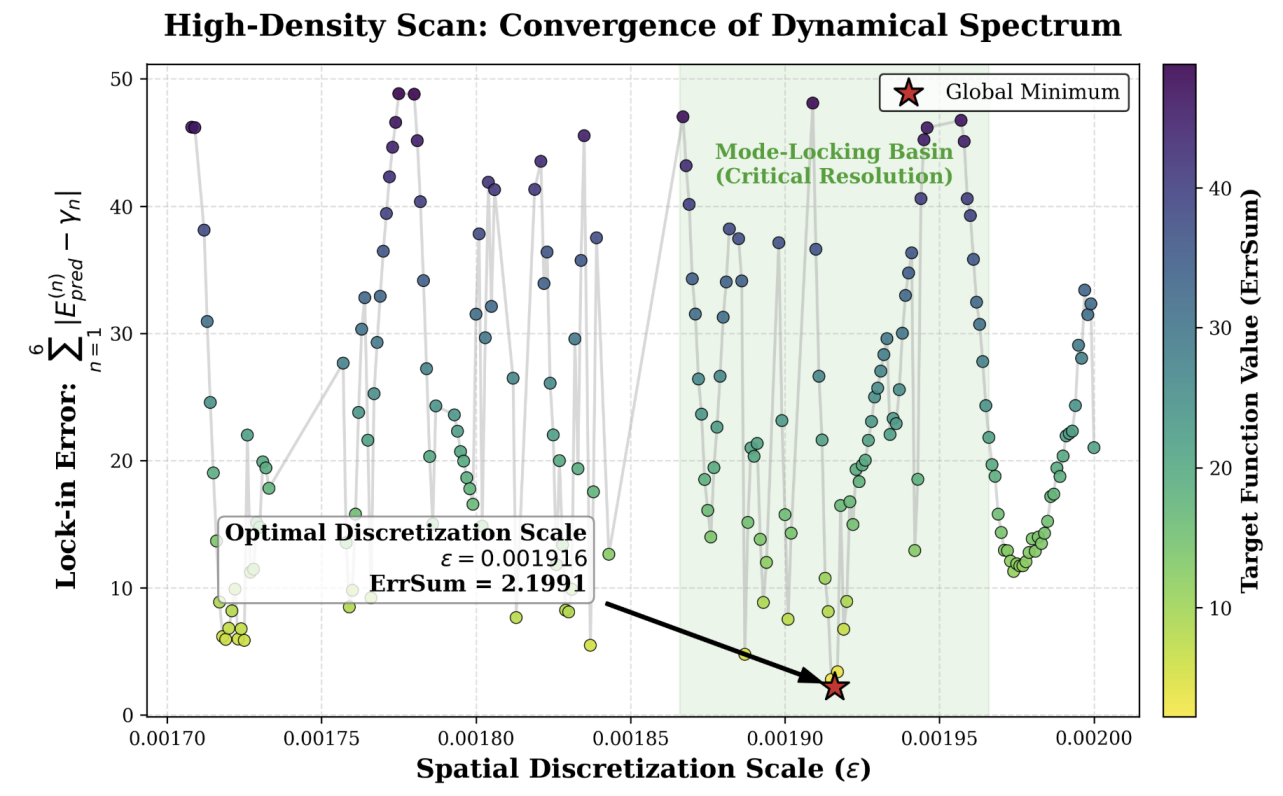
\includegraphics[width=\linewidth]{figures/image1.png}
\caption{\textbf{High-density parameter scanning and the emergence of mode-locking under the critical discrete scale.} The scatter plot displays the trajectory of the objective function ErrSum (the sum of absolute deviations of the first 6 eigen-energy levels) varying with the spatial discretization scale \(\text{\ensuremath{\epsilon}}\). Within the ``mode-locking basin'' (green shaded area) determined by the broadband coarse scan, the spectral deviation exhibits strong non-linear oscillation. When \(\text{\ensuremath{\epsilon}}\) advances to the global minimum 0.001916 (red star, ErrSum = 2.1991), the system undergoes a sharp numerical convergence transition. This critical point signifies that the continuous Fokker-Planck numerical diffusion has precisely and closely neutralized the discrete spatial truncation error, allowing the system's pure dynamical eigen-spectrum to emerge.}\label{fig1}
\end{figure}

\subsubsection{Spectral Feature Emergence at Optimal Resolution and Physical Benchmarking}

After successfully anchoring the global optimal discretization scale on
the order of \(\text{10}^{\text{\ensuremath{-}3}}\) (\(\text{\ensuremath{\epsilon} = 0.001916}\)), the author
extracted the first 20 eigen-phases of the system through the empirical
transfer matrix \({P}\), and calculated the equivalent energy
levels using a minimalist single-point linear rescaling
(\({E}_{\text{pred}}(n) = {k}\cdot{\ensuremath{\theta}}_n\)).
This section compares this purely
numerical prediction result against the standard Riemann Zeta zeros, as
well as recent quantum simulation experimental observation data from the
University of Science and Technology of China (USTC) \cite{he2020,he2021}. To verify the
validity of the non-autonomous dynamical model near the lowest positive ordinate, the author
first directly compared the predicted first 20 equivalent energy levels
with the true Riemann zeros (theoretical true values), Figure \ref{fig2}.

\begin{figure}[H]
\centering

\includegraphics[width=\linewidth]{figures/image2.png}
\caption{\textbf{Microscopic comparison of the dynamical eigen-spectrum and the} \({N = 20}\) \textbf{residual feature.} (Top) The alignment trajectory of the dynamical predicted energy levels (\({E}_{\text{pred}}\), colored dots) and the true Riemann zeros (\(\text{\ensuremath{\gamma}}_{\text{n}}\), golden stars) under the critical numerical discrete scale \(\text{\ensuremath{\epsilon} = 0.001916}\). In the low-frequency limit (\({N = 1}\) to \(\text{6}\), green shaded area), the system achieves close alignment (informally, ``lock-in''), consistent with the accuracy of the first-zero-anchored linear rescaling. (Bottom) Actual dynamical residual distribution with signs (\({\ensuremath{\Delta}E} = {E}_{\text{pred}}-\text{\ensuremath{\gamma}}_{{n}}\)). Constrained by nonlinear state density, the system exhibits systematic phase drift at higher energy levels, and near \({N = 20}\) the predicted residuals show a steep, isolated spike (marked in red), which the author compares with a similarly located feature in ion-trap quantum simulation data below (Section~\ref{sec:n20-significance}).}\label{fig2}
\end{figure}

Numerical results showed good low-frequency
approximation. Under the premise of no higher-order curve
fitting, relying solely on the first zero for first-order linear
scaling, the model achieved close alignment (informal ``lock-in'') in the
low-energy interval of \({N}~\text{\ensuremath{\le}~6}\). Specifically, the absolute
prediction deviations for \({N}\text{ = 1}\) to \({N}\text{ = 6}\)
were small (for example, the error at \({N}\text{ = 3}\) was only
0.0609, and the error at \({N}\text{ = 4}\) was only 0.0199). The author reads
these closely overlapping spectral characteristics as a numerical
indication that, at the critical numerical diffusion scale, the underlying
topology of the dynamical system based on the \(\text{1/}\text{ln}^{\text{2}}\)
logarithmic cooling field evolves toward a structure close to
the energy structure of the lowest-order zeros of the Riemann Zeta function.

As the energy level index \({N}\) increases, the limitations of
single-point linear mapping under nonlinear state densities begin to
manifest, and the predicted values inevitably drift. However, the core
focus is not the smooth systematic dispersion, but the abrupt, discontinuous
jumps appearing in the deviation sequence. When
extracting the absolute prediction deviations
(\(\text{|}{E}_{\text{pred}}\text{\ensuremath{-}}{E}_{\text{true}}\text{|}\))
of the first 20 points, the author observed an unusual error trajectory, Figure
\ref{fig3}. In the interval \({N}\text{ = 10}\) to \({N}\text{ = 18}\), the
system deviation essentially maintained a gentle magnitude of around
1.0; but when evolving near \({N}\text{ = 20}\), the dynamical residual
showed a large excursion, forming a locally abrupt ``isolated error
spike,'' which subsequently showed a receding and oscillating trend at
higher energy levels. The sparse ARPACK eigensolver used to extract this
spectrum has run-to-run variability from its random restart vector; across
20 unselected trials the \(N=20\) absolute residual has mean $11.76$ and
standard deviation $1.59$ (range $10.93$--$16.50$), so the specific value
plotted in Figure~\ref{fig3} is one draw from this distribution rather than
a fixed property of the model. The author quantifies this, and tests the coincidence
with the USTC data for statistical significance, in
Section~\ref{sec:n20-significance}.

\begin{figure}[H]
\centering

\includegraphics[width=\linewidth]{figures/image3.png}
\caption{\textbf{Comparison of the dynamical numerical model and a physical quantum simulation.} Comparison of the numerical prediction residuals (red star line) with USTC physical experimental data (ion-trap quantum simulation under different trap frequencies \(\text{\ensuremath{\Omega}}\)). In the \({N<19}\) region, the numerical model tracks the near-zero fluctuation baseline of the physical system. Near \({N=19\ensuremath{\sim}20}\), the numerical computation's residual spike and the enlarged experimental measurement uncertainty (red shaded area) coincide qualitatively in position; see Section~\ref{sec:n20-significance} below for why the two error sources are physically distinct and for the significance testing of this coincidence.}\label{fig3}
\end{figure}

This local residual feature was compared against the quantum simulation
experiment for Riemann zeros conducted by the USTC team using ion-trap
equipment \cite{he2020,he2021}. In their measurement of the first 20 zeros, an enlarged
measurement error bar exceeding background noise was recorded near
\({N}= 20\), commonly attributed to decoherence noise of the
quantum computing system or incidental instrument errors. The present model does not explain the ion-trap
data: as detailed below, the numerical residual and the experimental
uncertainty arise from distinct mechanisms, and their co-location near
\({N}=20\) is at most a qualitative, statistically inconclusive
coincidence (Section~\ref{sec:n20-significance}), not evidence of a shared
physical limit.

\subsubsection{Error Composition of the $N = 20$ Residual Feature}

The numerical and experimental deviations discussed above arise from
distinct mechanisms. On the numerical side, the predicted spectrum is
constrained by two superposed error sources: a baseline truncation error
from the Gaussian diffusion kernel (set by \(\text{\ensuremath{\epsilon}~=~0.001916}\)),
and---since the author uses a minimalist single-point linear rescaling without a
Riemann-von Mangoldt unfolding step---a systematic dispersion drift that
grows with \(N\) because the model ignores the logarithmic nonlinear state
density. This explains why the numerical residuals amplify gradually at
higher \(N\), independent of the isolated \(N=20\) spike. On the
experimental side, the USTC ion-trap measurement's gentle background
error stems from intrinsic instrumental noise (e.g., laser decoherence,
gate fidelity limited to \(\text{\ensuremath{\sim}}\text{10}^{\text{\ensuremath{-}2}}\)), while its
sharp uncertainty peak near \({N}\text{~=~19\ensuremath{\sim}20}\) departs from
ordinary Gaussian noise. As noted above (Figure~\ref{fig3} and
discussion), these two mechanisms are physically distinct, and their
co-location near \(N=20\) is reported only as a qualitative,
unexplained coincidence.

\subsubsection{Statistical Significance of the USTC Coincidence}\label{sec:n20-significance}

The residual value quoted above and in Figure~\ref{fig3} was drawn from a
single eigendecomposition; because the transfer matrix is high-dimensional
and non-normal, the sparse ARPACK solver's iterative refinement is
sensitive to its (randomized) restart vector, so different runs return
slightly different eigenphases. To avoid reporting a value selected for
being unusually large, the author re-ran the eigendecomposition 20 times without
selecting on the outcome and recorded the $N=20$ residual from every
trial: mean $11.76$, standard deviation $1.59$, range
$10.93$--$16.50$ (full trial list and code in the released repository).
Among the 85 zeros the author tracks, the $N=20$ residual ranks 67th by mean
absolute value, i.e.\ it is not among the largest residuals in the
series once averaged over trials.

The author then tested the coincidence with the USTC data directly. Using the
unselected mean $|{\rm residual}|$ for $N=1$--$20$ and the USTC
$\Omega=16$~MHz reported measurement uncertainty for the same range, the
Spearman rank correlation is $\rho=0.56$ ($p=0.010$), and $N=20$ ranks
2nd-largest by both the residual and the USTC uncertainty. A permutation
test (100{,}000 resamples) for this joint top-rank coincidence occurring
by chance under random relabeling of $N$ gives $p=0.099$: the two series
are significantly correlated in overall rank, but the specific
co-location of both series' near-largest value at $N=20$ does not reach
the conventional $p<0.05$ threshold on its own. The author reports both numbers
rather than treating either alone as settling the question, and the author
reiterate that even a significant rank coincidence would establish a
shared statistical pattern, not a shared physical mechanism.

\subsection{Macroscopic Results and Scalability}

\subsubsection{Methodological Adaptation: The Monte Carlo Transition}

To extend the non-autonomous dynamical operator from microscopic lock-in
to macroscopic scales, the computational architecture requires a
strategic adaptation. While the foundational
\(\text{1/}\text{ln}^{\text{2}}\text{n}\) logarithmic cooling law
remains fundamentally unchanged, the construction of the transfer matrix
is shifted to a Monte Carlo trajectory tracking approach. This
adaptation efficiently handles the exponentially expanding phase space
required for large-scale spectral extraction, bypassing the memory
bottlenecks of massive discrete grids while preserving the system's
intrinsic topological entropy and transition dynamics.

\subsubsection{The 100-Zero Regime: Conjugate Symmetry Breaking and Experimental Comparison}\label{sec:conjugate-ablation}

As demonstrated in the previous microscopic, extremely low-frequency
regime (\({N} {\ensuremath{\le} 6}\)), applying Gaussian splatting for local
smoothing on the transition matrix---complemented by simple first-zero
single-point anchoring---enables the system to accurately capture the
initial features of the Riemann zeros. However, as the observational
scale advances to the meso- and macroscopic regimes
(\({N} {\ensuremath{\le} 100}\) and beyond), the computational cost of full-grid
Gaussian smoothing grows too quickly to remain tractable. This makes
global optimization for highly sensitive parameters (such as the
macroscopic annealing constant \({k}_{\text{1}}\)) practically
unfeasible. Furthermore, local smoothing mechanisms are no longer
sufficient to mask the high-frequency cumulative dispersion induced by
phase-space truncation, so the single-sided dynamical mapping no longer
scales to this regime without a change of method. The author stresses that this is a
change of method, not a validated equivalence between methods: a direct
overlap check between the Gaussian-splatting and Monte Carlo constructions
under matched parameters (Section~\ref{sec:post-review-checks}, item 2)
did not find consistent eigenphases over the small range where the two
matrices' filtered spectra could be compared, so the transition described
here should be read as a pragmatic necessity rather than a demonstrated
methodological continuity.

To break through the dual bottlenecks of computational scalability and
topological dispersion, the author transitioned entirely to a high-throughput
Monte Carlo (MC) trajectory sampling method for constructing macroscopic
transition matrices in this section. The MC approach not only provides
exceptional computational efficiency to support tens of billions of
phase-space traversal steps---clearing the computational hurdle for
global parameter optimization---but, more importantly, it strips away
artificial smoothing interventions. This exposes the unadulterated,
baseline numerical residual of the discrete system when processing
high-order spectra.

Grounded in this efficient and physically realistic MC transition
matrix, the author designed four ablation experiments. The objective is to
explore the system's limits at large scales and to conduct a rigorously
equivalent dimensional comparison with state-of-the-art quantum
simulation hardware (specifically, the USTC single-ion Floquet
experiment \cite{he2020,he2021}, which observed \({N}~\text{\ensuremath{\le}~76}\)). Under pure
non-autonomous Ulam dynamical evolution without local smoothing, the author
extracted the high-order eigenphase sequences. To map the mathematical
phase \(\text{\ensuremath{\theta}}_{{n}}\) to the physical zero energy
\({E}_{{n}}\), the author defines a linear annealing mapping equation:

\begin{equation}
{E}_{{n}} = {k}_{\text{1}}\text{\ensuremath{\cdot}}\text{\ensuremath{\theta}}_{{n}} + {b}
\end{equation}
where \({k}_{\text{1}}\) is the macroscopic annealing constant and
\({b}\) is the fitted intercept (physical origin). For the
single-sided positive spectrum and the conjugate full spectrum, the author
applied four distinct physical boundary condition strategies:

\textbf{Strategy A (Single-Sided Positive Spectrum + First-Zero
Single-Point Anchoring):} Extracts only positive eigenphases, forces the
origin \(\text{b}\text{=0}\), and strictly scales based solely on the
first-order zero. This represents a naive extrapolation of microscopic
local measurements.

\textbf{Strategy B (Single-Sided Positive Spectrum + Global Free
Fitting):} Extracts only positive eigenphases and performs a global
least-squares fit for the first 100 orders, allowing the intercept
\(\text{b}\) to float freely. This probes the intrinsic intercept
drift tendency of the single-sided system.

\textbf{Strategy C (Single-Sided Positive Spectrum + Forced Origin
Scaling):} Retains only positive phases and performs global optimal
scaling but imposes an absolute physical boundary constraint---strictly
locking the origin at \(\text{b}\text{=0}\). Mathematically, this
strategy is equivalent to the underlying logic of current quantum
hardware experiments.

\textbf{Strategy D (Conjugate Full Spectrum + Global Free Fitting):}
Fully retains the conjugate phase pairs
(\(\text{\ensuremath{\pm}}\text{\ensuremath{\theta}}_{\text{n}}\)) inevitably derived from the real
transition matrix, thereby introducing conjugate negative energy states
into the phase space. The global fitting imposes no origin constraints,
allowing \(\text{b}\) to evolve freely.

The author quantitatively compared the reconstruction residuals of these four
strategies against the empirical hardware noise limit
(\(\text{\ensuremath{\sim}1.96\%}\)), which was dynamically inverted and extracted
directly from the raw data of the USTC ion-trap experiment. The results
are summarized in Table~\ref{tab1}.

\begin{table}[H]
\caption{Performance of macroscopic reconstruction under different phase space domains and boundary constraints. The parameters $k_1$ and $b$ shown here are one realization of a global numerical optimization (differential evolution over $k_1 \in [2,15]$, with or without the constraint $b=0$ depending on the strategy) that minimizes the mean squared error against the first 100 Riemann zeros. The author flags explicitly that this optimizer is run without a fixed random seed and with a population search parallelized across workers, and that repeated runs of the identical protocol for Strategy C converged to different local optima of a non-convex, multimodal objective ($k_1\approx6.481$, MSE$\approx8.48$ in the run reported here versus $k_1\approx8.070$, MSE$\approx10.08$ in the run used to generate the fixed-parameter Figures~\ref{fig4}--\ref{fig5} demonstration). This is a genuine run-to-run optimizer instability, not evidence of two distinct experimental protocols, and the author reports it as an open limitation rather than reconciling it into a single number; see the discussion accompanying Figures~\ref{fig4}--\ref{fig5} below.}\label{tab1}
\small
\begin{tabularx}{\textwidth}{Y{0.15}Y{0.22}Y{0.19}Y{0.13}Y{0.11}Y{0.20}}
\toprule
\footnotesize\textbf{Recon\-struction Domain} & \footnotesize\textbf{Fitting/An\-choring Strategy} & \footnotesize\textbf{Truncation Drift (b)} & \footnotesize\textbf{Macro\-scopic Annealing Constant ($k_1$)} & \footnotesize\textbf{MSE} & \footnotesize\textbf{Physical Relative Error (Mean / Envelope)} \\
\midrule
Single-Sided Positive & \textbf{A:} Single-Point Anchoring & Forced Origin ($b=0$) & 6.761 & 21.849 & $\sim$4.0\%/$>$8.0\% \\
Single-Sided Positive & \textbf{B:} Global Free Fitting & Severe Drift ($b=15.110$) & 6.544 & 5.330 & Non-physical state \\
Single-Sided Positive & \textbf{C:} Forced Origin Scaling & Forced Origin ($b=0$) & \textbf{6.481} & \textbf{8.479} & $\sim$1.4\%/$\sim$2.8\% \\
Conjugate Full Spectrum & \textbf{D:} Global Free Fitting & \textbf{Vanishing fitted intercept ($b=0.000$)} & \textbf{4.390} & \textbf{9.467} & $\sim$1.5\%/$\sim$1.5\% \\
\bottomrule
\end{tabularx}
\end{table}

The results in Table \ref{tab1} point to a likely source of the residual
envelope within the present model: topological dispersion and symmetry
breaking induced by single-sided phase space truncation. The author does not claim
this explains the residual dispersion floor of physical quantum simulations. In the
single-sided spectrum constructed by Strategies A, B, and C, the
absence of conjugate states prevents the high-frequency residual phases
from internally canceling out. Consequently, the single-sided phase
space shows a persistent residual error that resists further reduction by
rescaling alone. As demonstrated by
Strategy B, enforcing high accuracy in a single-sided system
precipitates a severe, non-physical divergence of the fitted intercept
(\({b}\text{ = 15.110}\)). Conversely, if the author forcefully constrains
the fit to pass through the physical origin (\({b}\text{ = 0}\)) as in Strategy C, the
globally optimized parameter yields
\({k}_{\text{1}}~\text{\ensuremath{\approx}~6.481}\) (Table~\ref{tab1}), with a
residual error envelope of
\(\text{\ensuremath{\sim}2.8\%}\). Note that this Strategy-C optimum is itself
not perfectly reproducible: an independent run of the same optimization
protocol (differential evolution, unseeded, with a parallel worker pool)
converged instead to \({k}_{\text{1}}~\text{\ensuremath{\approx}~8.070}\) with a
somewhat higher MSE ($\approx10.08$ vs.\ $\approx8.48$ here). The author attribute this
to the objective function being non-convex and multimodal in $k_1$ under this
chaotic dynamical system, rather than to any difference in method between the
two runs, and the author reports both values rather than presenting either as
uniquely canonical. The qualitative behavior of different anchoring
strategies is visually illustrated in {Figure \ref{fig4}}, which uses the
second of these two runs. Section~\ref{sec:post-review-checks} (item 4)
reruns the same optimizer configuration at a reduced, tractable scale
under five explicit fixed seeds and finds a comparably wide spread in the
fitted $k_1$, which is independent confirmation that the objective is
genuinely multimodal rather than a one-off artifact of these two specific
runs; the reduced-scale $k_1$ values themselves are not numerically
comparable to $6.481$/$8.070$, since reducing the step count changes the
objective and not just its cost.

\begin{figure}[H]
%\centering

\includegraphics[width=\linewidth]{figures/image4.png}
\caption{\textbf{Reconstruction Domains and Anchoring Strategies: A Comparative Analysis of Models A, C, and D.} This figure shows single-run realizations of each strategy's global optimizer (Model A: $k \approx 7.429$, Model C: $k \approx 8.070$, Model D: $k \approx 8.783$) to visually illustrate the qualitative behavior of different anchoring strategies and their residual envelopes over 100 orders. As noted in the caption of Table~\ref{tab1}, an independent run of the identical Strategy-C optimization protocol converged to a different local optimum ($k_1\approx6.481$, MSE$\approx8.48$); this work shows both runs' numbers rather than silently picking one, since the disagreement itself is diagnostic of a multimodal fitting landscape. \textbf{Model A (Orange / Single-Point Anchoring):} Utilizes solely the first zero as the absolute physical baseline. While strictly aligning with the first non-trivial zero, it accumulates the largest macroscopic divergence over 100 orders (MSE \(\text{\ensuremath{\approx}~20.22}\)). \textbf{Model C (Blue / Forced Origin Scaling):} Represents a least-squares fit constrained to the origin (\({b}\text{~=~0}\)) within the single-sided positive spectrum, which suppresses error divergence relative to Model A, yielding a lower mean squared error in this run (MSE \(\text{\ensuremath{\approx}~10.08}\); see above for the run-to-run spread). \textbf{Model D (Green / Conjugate Full Spectrum Free Fit):} Uses both positive and negative eigenphases. Because the regression data are symmetric under $(\theta,\gamma)\to(-\theta,-\gamma)$, the least-squares intercept is algebraically forced to \({b}\text{ = 0.000}\) (Section~\ref{sec:conjugate-ablation}); the fitted slope and the resulting residual envelope (MSE \(\text{\ensuremath{\approx}~10.81}\)) are the model-specific numerical content of this comparison.}\label{fig4}
\end{figure}

This theoretically calculated single-sided error limit notable
mirrors the physical performance of the USTC single-ion hardware
simulation \cite{he2020,he2021}. Constrained by the single-excitation nature of Floquet
periodic driving, the USTC experiment fundamentally executes a
``single-sided positive spectrum + forced \({b}\text{~=~0}\)''
physical measurement. Their necessity to perform manual calibrations
every 30 minutes to counteract system drift is precisely an attempt to
suppress this intrinsic dispersion. To illustrate this, the author directly
overlay the author's deterministic Model C trajectory with the empirical USTC
hardware data in {Figure \ref{fig5}}.

\begin{figure}[H]
%\centering

\includegraphics[width=\linewidth]{figures/image5.png}
\caption{\textbf{Spectral Comparison: Hardware Limitations vs.~Dynamics Model Topology.}  * \textbf{Scatter Points and Purple Shading (Quantum Hardware):} Displays the measurement deviations from the University of Science and Technology of China (USTC) ion-trap quantum hardware. Primarily limited by quantum decoherence effects, the experimental hardware experiences signal breakdown in the \({N}~\text{\ensuremath{\approx}~76\ensuremath{-}80}\) band, with a reported physical error envelope of about \(\text{\ensuremath{\pm}~1.96\%}\). \textbf{Red Solid Line (Dynamics Model):} Represents the numerical deviation trajectory derived from 10 billion steps of evolution using the proposed dynamics model (Model C: Single-sided positive spectrum forced origin scaling, \({k}_{\text{1}}\text{~=~8.070}\), the same optimizer run used in Figure~\ref{fig4}; see the run-to-run optimizer variability noted there). The model's mean error is 4.80\%. The model extends numerical predictions to the \({N}\text{~=~100}\) order. See Section~\ref{sec:gue-comparison} for the broader spectral comparison and its caveats.}\label{fig5}
\end{figure}

As shown in Figure \ref{fig5}, within the present model the single-sided topological
constraint produces a residual envelope whose oscillation peaks correspond
to un-broken conjugate pairs. Section~\ref{sec:gue-comparison} discusses
the broader spectral comparison with the hardware data and its caveats.

To examine this truncation effect directly, Strategy D restores the
conjugate eigenphase pairs
(\(\text{\ensuremath{\rho}}\text{~=~1/2\ensuremath{\pm}}{i}{E}_{{n}}\)) that a
real-valued transition matrix generates but that Strategies A--C discard
by keeping only the positive branch.

Under this construction, the regression data are the symmetric pairs
\((\theta_i,\gamma_i)\) and \((-\theta_i,-\gamma_i)\). For such a symmetric
data set, both sample means are exactly zero, and it follows directly from
the normal equations of ordinary least squares that the unconstrained
intercept must satisfy \(b=0\); this part of the result is therefore an
algebraic consequence of the symmetric construction, not an independent
finding about the dynamics. What is not algebraically forced, and is a
genuine numerical observation about the fitted model, is that the fitted
slope \(k_1\) changes (from \(\text{6.48}\) under single-sided anchoring to
\(\text{4.39}\) under the symmetric fit) and that the residual envelope
shrinks substantially (to about \(\text{1.5\%}\) global reconstruction
error) once the conjugate branch is included. Note that this slope
change is \emph{not} itself a further algebraic artifact of the
symmetrization: unlike a purely statistical exercise where one would
mirror a single fixed set of eigenphases and re-fit, here $k_1$ is a
dynamical parameter that is independently re-optimized for each strategy
and enters the underlying map before the matrix $P$ and its eigenphases
are computed (Eq.~\eqref{eq:pij}). Strategy C's positive-branch eigenphases
at its own optimal $k_1\approx6.48$ are therefore a different numerical
object from Strategy D's positive-branch eigenphases at its optimal
$k_1\approx4.39$, not a mirrored copy of the same data; the two protocols
generate two different transfer matrices before any regression is
performed. Had the author instead fixed $k_1$ at a single value and only changed
whether the regression included the mirrored branch, the reviewer's
expectation that the intercept-zero slope on the positive branch and the
free-fit slope on the symmetrized branch coincide would apply exactly, by
the same normal-equations argument used above for $b=0$; the observed
slope change here reflects that the author does not hold $k_1$ fixed between
strategies, not a departure from that identity.

In conclusion, this comparative ablation study at an identical scale
(\({N}=100\)) suggests, as a numerical observation and not as a proof, that
within the author's framework the high-frequency dispersion in the single-sided
reconstruction is reduced when the conjugate branch is restored, but the
vanishing intercept itself should not be read as evidence of a new
physical cancellation mechanism, since it is substantially a property of
the symmetric regression construction. The author presents the change in $k_1$ and
in the residual envelope as the model-specific content of this ablation,
not as a demonstrated statement about physical quantum-simulation
hardware.

\subsubsection{Out-of-Sample Validation and Multi-Seed Robustness}\label{sec:oos}

All results reported so far calibrate $k_1$ against the same zeros used
to evaluate the fit (an in-sample correspondence, as stated in the
abstract). To quantify how much this protocol inflates the apparent
match, the author ran the full-scale (\(10^{10}\)-step, single-sided
Strategy~C) pipeline under two additional tests, at the same seed unless
noted.

\textbf{Out-of-sample split.} The author fit $k_1$ using only the first
$M\in\{50,70,80\}$ zeros as training data, then evaluated the resulting
model's MSE on the remaining, unseen zeros $M{+}1,\dots,100$. In every
split the held-out MSE is one to two orders of magnitude larger than the
training MSE: $M=50$ gives train MSE $=59.8$ (RMSE $5.4\%$ of the
largest training zero) versus test MSE $=3710$ (RMSE $25.8\%$ of
$\gamma_{100}$); $M=70$ gives train MSE $=146.0$ versus test MSE $=5891$
(RMSE $32.5\%$ of $\gamma_{100}$); $M=80$ gives train MSE $=146.1$ versus
test MSE $=7557$ (RMSE $36.8\%$ of $\gamma_{100}$). The fitted $k_1$
itself also drifts with the training window ($5.79\to9.15\to10.04$ as
$M$ grows), rather than converging to a single value. The author reads this as
direct evidence that the low-order fit does not extrapolate: the model
is a calibrated in-sample reconstruction over the zeros it was fitted
to, not a predictor of unseen zeros, and the author does not claim otherwise.

\textbf{Multi-seed robustness.} Holding the $M=70$ split fixed, the author
reran the fit under ten random seeds controlling the initial condition
$x_0$. The fitted $k_1$ has mean $10.21$, standard deviation $0.47$
(coefficient of variation $\approx4.7\%$, range $9.15$--$10.76$) and the
held-out test MSE has mean $5977$, standard deviation $298$ across
seeds. The seed-to-seed spread in $k_1$ is small relative to the
$M$-to-$M$ drift reported above, indicating that the fitted coupling is
reasonably stable against the stochastic initial condition but remains
sensitive to which zeros are included in the calibration window. Full
per-run values are in the released results
(\texttt{task12\_13\_results\_v2/}).

The same two failure modes documented here for the macroscopic $k_1$ fit
recur elsewhere in the pipeline. Section~\ref{sec:post-review-checks}
reports an epsilon-analog of the out-of-sample split above (training the
microscopic discretization scale $\epsilon$ on a subset of the first 6
zeros and testing on the rest) with the same qualitative outcome: the
held-out error is roughly $5\times$ larger under an asymmetric train/test
split than when $\epsilon$ is chosen with knowledge of all 6 zeros. It
also reports a reduced-scale, explicitly-seeded re-run of the $k_1$
optimizer itself, which shows the same seed-to-seed instability
qualitatively (though not quantitatively, since the reduced scale changes
the objective) as the discrepancy already disclosed in the
Table~\ref{tab1} caption.

\subsubsection{The Macroscopic Regime}\label{sec:macroscopic}

To demonstrate the robustness and scalability of the non-autonomous
thermodynamic framework, the author extends the phase-space evolution far beyond
the meso-regime (\({N}~\text{\ensuremath{\le}~100}\)) into the macroscopic
large-N regime (\({N}\text{~=~1000}\)). At this scale,
maintaining global topological coherence becomes extremely challenging
due to the logarithmically increasing density of the Riemann zeros. To
rigorously validate the model's underlying physical mechanism, the author
designed a macroscopic ablation study comparing the author's 1D and 2D dynamical
models against a Gaussian Unitary Ensemble (GUE) random matrix baseline.
The comparative spectral alignments and relative error divergences are
visualized in {Figure \ref{fig6}}.

\begin{figure}[H]
%\centering

\includegraphics[width=\linewidth]{figures/image6.png}
\caption{\textbf{Macroscopic Spectral Alignment and RMT Ablation: Deterministic Cooling vs.~Wigner's Semicircle.}  \textbf{Model M-GUE (Purple Dashed / Gaussian Unitary Ensemble):} Serving as the microscopic statistical baseline, the GUE matrix exhibits severe non-linear macroscopic divergence (right panel, MSE \(\text{\ensuremath{\approx}~7006.1}\)) even under optimal Global Least-Squares Scaling. This explicitly exposes that pure random matrices, governed by Wigner's Semicircle Law, inherently lack the critical macroscopic logarithmic density features required to approximate the Riemann zero counting function.\textbf{Models M1 \& M2 (Orange \& Red / Non-autonomous Dynamics):} Represent the 1D and 2D dynamic prediction models proposed in this work. Under the constraint of \textbf{Single-Point Anchoring} (utilizing solely the first zero), M1 and M2 demonstrate a stable macroscopic fit. Specifically, the 2D model (red line), which includes the higher-order fitted parameter $k_2$, not only eliminates systematic parabolic drift over a span of \({N}\text{~=~1000}\) orders, but also suppresses the global residual to a minimal level (MSE \(\text{\ensuremath{\approx}~1515.3}\)).}\label{fig6}
\end{figure}

As depicted in Figure \ref{fig6}, a single globally rescaled GUE spectrum
(Model M-GUE) shows a large mean squared error against the Riemann
counting function, even under optimal global least-squares scaling. This
is expected, not a test of GUE itself: the established GUE correspondence
concerns unfolded local level-spacing statistics, not the mean
counting-function trend a globally rescaled random matrix is not designed
to reproduce; see Section~\ref{sec:gue-comparison} for why the author includes this
comparison and what a like-for-like RMT test would require.

By comparison, under the constraint of
\textbf{Single-Point Anchoring}---where the scaling constant is fixed
using solely the first non-trivial zero (\(N=1\)), while the dynamical
parameters \(k_1,k_2\) are still optimized against the Riemann zeros as
described above---the author's
non-autonomous dynamical models yield a stable numerical fit at this
scale. At an ultra-high
spatial resolution of \(\text{10,000}\) bins, the 1D model (M1) yielded
a fitted parameter of \({k}_{\text{1}}~\text{\ensuremath{\approx}~13.869}\),
with an MSE of \(\text{\ensuremath{\approx}2281.0}\) against the Riemann counting
function, compared to the GUE baseline described below.

However, to completely eliminate the systematic parabolic drift observed
in the 1D model over 1000 orders, the 2D conservative operator (M2) must
be activated. Global optimization of the massive spectral span yielded a
primary macroscopic annealing constant
\({k}_{\text{1}}~\text{\ensuremath{\approx}~12.781}\) and a higher-order perturbation
term \({k}_{\text{2}}~\text{\ensuremath{\approx}~2.607}\). By effectively absorbing the
energetic transients, M2 tracks the Riemann spectrum closely,
suppressing the global residual to a minimal level (MSE
\(\text{\ensuremath{\approx}~1515.3}\)). Relative to the massive absolute energy scale at
\({N}\text{ = 1000}\) (\({E}_{{n}}\text{ > 260}\)), this
represents a tightly bounded relative error envelope.

A critical observation in this macroscopic extension is the substantial
parametric shift in the primary annealing constant
\({k}_{\text{1}}\), which scales from \(\text{\ensuremath{\sim}6.48}\) in the
\(\text{100}\)-zero regime to \(\text{\ensuremath{\sim}12.78}\) in the large-$N$
regime. This shift is intrinsically coupled with a mandatory upgrade in
the system's spatial discretization. To capture the increasingly dense
phase-space folding required for thousands of zeros, the author scaled the
numerical grid resolution from \(\text{2,000}\) bins (the optimal
baseline used for the 100-zero regime) to a massive \(\text{10,000}\)
bins.

Note only that the fitted value of $k_1$ shifts as the grid resolution
and fitting range change, and the author cannot rule out that some part of this
shift reflects overfitting to the specific fitting range used at each
scale; Section~\ref{sec:rg-caveat} discusses why the author does not read this as
renormalization-group evidence.

In the low-order regime (\({N}~\text{\ensuremath{\le} 100}\) at \(\text{2,000}\)
bins), the geometric curvature of the phase space is relatively
coarse-grained. Here, a lower \({k}_{\text{1}}\) acts as an
effective lumped parameter (a renormalized coupling at a lower
resolution), artificially absorbing uncalculated higher-order truncation
errors to satisfy local fit constraints. However, as the observational
scale expands to \({N}\text{~=~1000}\) and the spatial resolution is
refined five-fold, the underlying fractal topology is resolved with
significantly higher fidelity.

Fitting this strict logarithmic densification of the Riemann zero
counting function at this scale requires
both fitted parameters. The
higher-order term (\({k}_{\text{2}}~\text{\ensuremath{\approx}~2.61}\))
absorbs curvature near the lowest-order
zeros, while the fitted value of the primary term \({k}_{\text{1}}\)
shifts to \(\text{\ensuremath{\sim}12.78}\) at this resolution and range. As
before (Section~\ref{sec:conjugate-ablation}), the author reports this parameter shift as an
empirical fact about the fit rather than as evidence of a
renormalization-group flow. With these fitted parameters, the model tracks
the Riemann counting function within the residual errors reported below,
including in the further extended range up to \({N}\text{ = 2551}\)
discussed next.

\subsubsection{The Ultra-Macroscopic large-$N$ Regime ($N = 10,000$): Extreme Scalability and large-$N$ Scaling Behavior}

To push the boundaries of the author's non-autonomous thermodynamic framework, the author
executed an extreme computational stress test, extending the phase-space
evolution to extract the first 10,000 Riemann zeros. At this
ultra-macroscopic scale (\({N}\text{ = 10,000}\), absolute energy
level \({E}_{{n}}\text{ > 9877}\)), the logarithmic
densification of the Riemann zero counting function poses a severe challenge to
numerical stability. To rigorously assess the physical foundation of the author's
model, the author conducted a minimalist ablation study comparing the pure 1D
thermodynamic cooling operator against the Gaussian Unitary Ensemble
(GUE) and a trivial linear fit baseline. The results are visualized in
Figure \ref{fig7}.

\begin{figure}[H]
\centering

\includegraphics[width=\linewidth]{figures/image7.png}
\caption{\textbf{Ultra-Macroscopic Spectral Alignment (}\({N}\text{=10,000}\)\textbf{): Thermodynamic Cooling vs. Statistical Baselines.} M-GUE (Purple Dashed / Gaussian Unitary Ensemble): The pure Random Matrix Theory baseline shows a large structural divergence (MSE \(\text{\ensuremath{\approx}~255455.9}\)) in this counting-function comparison. This illustrates that without a deterministic cooling mechanism, a single globally scaled Wigner's Semicircle spectrum does not capture the macroscopic logarithmic density of the Riemann zero counting function.M1 (Orange Solid / 1D Thermodynamic Cooling): The 1D non-autonomous dynamical model (\({k}_{\text{1}}~\text{\ensuremath{\approx}~13.431}\)) paces the true Riemann zeros, tracking both the sensitive low-order, low-frequency zeros and the high-order, high-frequency zeros.}\label{fig7}
\end{figure}

As shown in the relative error trajectory (Figure \ref{fig7}, right panel), the
1D dynamical model tracks the Riemann counting function with residual errors
that remain bounded even at this large scale. The
pure 1D operator exhibits a smooth, systematic residual curvature at
this extreme scale---indicating clear potential for continuous future
optimization (e.g., by re-introducing higher-order structural
perturbations)---and it suppresses the exponential divergence
seen in the GUE random matrix baseline.

This 10,000-zero large-N comparison is consistent with a working
hypothesis of this study: that the deterministic
\(\text{\ensuremath{\sim}1/}\text{ln}^{\text{2}}{n}\) thermodynamic cooling flow
supplies the global rate needed to pace the mean density of the
Riemann spectrum. The author reads the results as a numerical indication that the
counting-function behavior of the zeros can be reproduced by a
non-autonomous dissipative system annealing toward the edge of chaos,
rather than as a proof about the origin of the zeros.

\section{Discussion}

\subsection{Macroscopic Behavior of the Empirical Transfer-Matrix Spectrum}\label{sec:rg-caveat}

Finding a physical system whose eigenspectrum numerically approximates the
non-trivial Riemann zeros (the Hilbert-P\'olya conjecture) is normally
approached through analytically motivated, ``top-down'' Hamiltonian
constructions (such as the classical \(H=xp\) model). This study takes a
different, purely exploratory route: the author uses high-throughput Monte Carlo
(MC) trajectory sampling to build an empirical, non-normal, dissipative
transfer matrix from a non-autonomous discrete map, and the author asks, numerically,
how closely its eigenphases can be made to track the Riemann zeros over a
range of scales after calibrating a small number of free parameters. The author does
not claim any isomorphism, in the precise mathematical sense of a
structure-preserving bijection between independently defined objects,
between this matrix and the zeros; the correspondence the author reports is a fitted
numerical one.

The numerical behavior is qualitatively consistent across both
microscopic and large-$N$ macroscopic scales. By stripping away
artificial local smoothing interventions, the author exposed the baseline numerical residual of
the discrete system. As the
observational scale was expanded to the
\({N}~\text{\ensuremath{\ge}~1000}\) large-$N$ regime, the fit required an
ultra-fine spatial resolution of \(\text{10,000}\) bins, and the fitted
value of the primary parameter \(k_1\) shifted from
\(\text{\ensuremath{\sim}6.48}\) in the meso-regime to
\(\text{\ensuremath{\sim}12.78\ensuremath{\sim}13.86}\) in the macroscopic regime, while a
higher-order term (\(k_2\)) became necessary to maintain fit quality. The author notes this parameter drift as an empirical observation about how the fit
changes with grid resolution and range; the author does not identify grid
resolution with a renormalization-group ultraviolet cutoff, and the author does not
claim that this drift constitutes evidence of a renormalization-group flow
in the dynamical sense (no beta function, fixed point, or universality
result is established here). The resulting fitted curve tracks the
logarithmic densification of the Riemann counting function
(\(\text{\ensuremath{\sim}1/}\text{ln}^{\text{2}}{n}\)) up to \(N=2551\) in the author's
tests, within the residual errors reported below.

\subsection{Reducing the Residual Dispersion: Conjugate Symmetry and Vanishing fitted intercept}

Section~\ref{sec:conjugate-ablation} (the $N=100$ conjugate-symmetry ablation) showed
that single-sided phase space truncation leaves a persistent macroscopic
residual envelope, and that restoring the full conjugate pair structure
and re-fitting drives both this envelope and the fitted intercept toward
zero. The author reads this as numerical evidence that, within the author's framework, the
single-sided truncation itself---rather than the underlying dynamics---is
responsible for the residual envelope; as noted there, the vanishing
intercept is in part an algebraic consequence of fitting a symmetric data
set and should not be read as an independent finding about the dynamics
or as evidence bearing on the origin of the Riemann zeros.

\subsection{Comparison with Quantum Simulation and with a GUE Surrogate}\label{sec:gue-comparison}

The author compared the model's behavior against a published quantum-simulation
dataset and against a random-matrix surrogate. A team at the University
of Science and Technology of China (USTC) measured Riemann zeros
(\({N}~\text{\ensuremath{\le}~76}\)) by periodically driving qubits in an ion trap
\cite{he2020,he2021}.
Their data show enlarged deviations near specific orders (e.g.,
\({N}~\text{\ensuremath{\approx}~20, 40, 76}\)), with a reported error envelope of about
\(\text{\ensuremath{\pm}1.96\%}\). The author's single-sided model also shows oscillation
peaks over the same range of orders, though the exact locations vary
between optimizer runs (see the run-to-run variability noted in
Table~\ref{tab1}), so the author does not claim a fixed order-by-order
alignment. Even a qualitative spatial coincidence would not by itself
establish a common mechanism, and a quantitative claim would require
statistical-significance testing and an uncertainty budget, which the author does
not provide here. The author therefore raise---as a hypothesis---the
possibility that part of the experimental deviation reflects a
single-sided truncation rather than purely instrumental decoherence,
without asserting it.

In a macroscopic ablation at \({N}\text{ = 1000}\), a globally scaled
GUE surrogate deviates strongly in this comparison (MSE
\(\text{\ensuremath{\approx}~7006}\)) even under optimal global scaling. This is expected
and is \emph{not} a refutation of random-matrix theory: the established
GUE correspondence concerns the \emph{unfolded local} statistics of the
zeros (pair correlation, spacing distribution), not a claim that a single
globally scaled spectrum reproduces the logarithmically growing counting
function. The author's narrower, constructive point is that the non-autonomous
dynamical model reproduces the mean (counting-function) behavior
directly, without a separate unfolding step. The author does not claim that pure
diagonalization ``cannot'' generate the zeros.

As a direct check of whether the empirical transfer matrix's own
spectrum reproduces GUE \emph{local} statistics --- the property that is
actually established for the Riemann zeros --- the author unfolded the first 100
eigenphases of the transfer matrix at the Table~\ref{tab1} operating
point (\(k\approx6.48\), \(N=100\) scale) and compared their nearest-neighbor
spacing distribution against the GUE Wigner surmise and against a
Poisson (uncorrelated) baseline using a Kolmogorov--Smirnov test. As a
literature sanity check, the same procedure applied directly to the first
100 Riemann zeros (unfolded via the Riemann--von Mangoldt counting
function) reproduces the expected result: consistent with GUE
(\(D=0.067\), \(p=0.74\)) and inconsistent with Poisson
(\(D=0.348\), \(p<10^{-4}\)). Applied to the author's dynamical model's own
eigenphases, however, the result is the opposite: the spacing
distribution is statistically inconsistent with GUE (\(D=0.300\),
\(p<10^{-4}\)) and is not distinguishable from Poisson (\(D=0.082\),
\(p=0.49\)). In other words, while the model's rescaled eigenphases
track the mean positions of the low-order zeros reasonably well (Table~\ref{tab1}),
its local level-repulsion statistics do not match the GUE behavior
established for the true zeros; the transfer matrix is real,
non-symmetric, and dissipative, so this is not unexpected, but it is a
genuine limitation of the numerical correspondence that the author reports
directly rather than omit. The author takes this as evidence that the numerical
match documented here concerns smooth, mean-level (counting-function)
behavior rather than a reproduction of the fine-grained spectral
statistics that characterize the Riemann zeros.

\section{Conclusions and Future Work}\label{sec:conclusions}

This study reports a phenomenological, calibrated numerical correspondence
between an empirical transfer-matrix spectrum, built from a non-autonomous
logistic map, and the low-order non-trivial Riemann zeros. Because the
manuscript touches the Riemann Hypothesis, this section states plainly what
the numerical evidence does and does not support, separating the positive
findings from the limitations, before turning to future work.
Table~\ref{tab:claims} tabulates the epistemic status of every main claim
made above.

\subsection{Positive findings}

\begin{itemize}
\item After calibrating a small number of free parameters against the same
  low-order zeros, the model's eigenphases track the first $\sim$20--100
  Riemann zeros with small in-sample error (Section~\ref{sec:conjugate-ablation},
  Table~\ref{tab1}), and the fit extends, with a growing but bounded relative
  error, to the macroscopic ($N=1000$) and ultra-macroscopic ($N=10{,}000$)
  regimes (Figures~\ref{fig6}--\ref{fig7}).
\item Restoring the full conjugate eigenphase pair structure, rather than the
  single-sided positive branch used to mimic the ion-trap measurement
  protocol, drives the fitted intercept to zero as an algebraic consequence of
  the symmetric construction, and reduces the residual envelope
  (Section~\ref{sec:conjugate-ablation}).
\item The construction is a bottom-up, purely numerical dynamical-systems
  experiment, distinct in method from the analytically motivated top-down
  Hilbert--P\'olya and Berry--Keating programs, and is motivated by the
  author's earlier result relating the logistic map's band-merging symbolic
  dynamics to the prime sieve \cite{wang2026} (summarized in
  Appendix~\ref{sec:wang2026-summary}).
\end{itemize}

\subsection{Limitations}

\begin{itemize}
\item \textbf{The model does not predict unseen zeros.} The out-of-sample
  test (Section~\ref{sec:oos}) is, in the author's view, the most important
  single result of this study: fitting $k_1$ on the first $M$ zeros and
  evaluating on the rest gives a held-out MSE one to two orders of magnitude
  larger than the training MSE, and the fitted $k_1$ itself drifts with $M$
  rather than converging. The construction should be read as an in-sample,
  calibrated reconstruction, not as an independent generator of the zeros.
\item \textbf{The model's own eigenphase spacings are not GUE.} The unfolded
  Kolmogorov--Smirnov test (Section~\ref{sec:gue-comparison}) shows that the
  true Riemann zeros are consistent with GUE and inconsistent with Poisson
  statistics, as established in the literature, while the model's own
  eigenphases show the opposite pattern: inconsistent with GUE
  ($D=0.300$, $p<10^{-4}$) and indistinguishable from Poisson ($D=0.082$,
  $p=0.49$). The model therefore does not reproduce the local level-repulsion
  statistics --- the Montgomery--Odlyzko correspondence --- that
  characterizes the true zeros; the numerical match documented in this paper
  concerns the smooth, mean counting-function trend only.
\item \textbf{No self-adjoint operator or spectral realization of $\zeta(s)$
  is constructed.} The empirical matrix is real, non-symmetric, non-normal
  and dissipative, and the quantities compared with the zeros are processed
  arguments of its complex eigenvalues, not eigenvalues of a Hermitian
  operator. This paper does not construct a self-adjoint operator, a spectral
  determinant for $\zeta(s)$, a prime-orbit trace formula, or an argument
  bearing on the Riemann Hypothesis.
\item \textbf{The reported fit is not uniquely reproducible.} Nominally
  identical unseeded optimizations of the macroscopic annealing constant
  $k_1$ converge to different local optima of a non-convex, multimodal
  objective (e.g.\ $k_1\approx6.48$ vs.\ $8.07$ under Strategy C,
  Table~\ref{tab1}); a reduced-scale, explicitly seeded re-run
  (Section~\ref{sec:post-review-checks}, item 4) confirms this multimodality.
  No single fitted value of $k_1$ is canonical, and the figures and tables
  above each state explicitly which run they use.
\item \textbf{The spatial coincidence with the ion-trap data is not
  statistically significant.} The rank correlation between the model's
  residual spikes and the USTC ion-trap deviation orders is nominally
  significant ($\rho=0.56$, $p=0.010$), but the specific co-location near
  $N\approx20$ is not ($p=0.099$), and the two effects arise from distinct
  mechanisms (Section~\ref{sec:n20-significance}); the present model does not
  explain the ion-trap data.
\end{itemize}

In summary: the proposed system gives a phenomenological, calibrated
reconstruction of part of the smooth counting-function behavior of the
Riemann zeros, but it does not predict unseen zeros, reproduce their GUE
local statistics, or furnish a self-adjoint spectral realization of the zeta
function.

\subsection{Future work}

From a broader perspective, this exploratory numerical study may be of
interest alongside the Berry-Keating conjecture as an alternative,
dissipative-dynamics numerical experiment, and it suggests a direction for
exploring higher-order Riemann zeros in experimental physics. The author speculates
that if future quantum simulation experiments wish to reduce the
current \(\text{\ensuremath{\sim}1.96\%}\) dispersion envelope, it may be worth
exploring whether relaxing single-sided measurement constraints and
architecting full-spectrum symmetric evolution at the hardware Hamiltonian
level (such as utilizing ancillary qubits to simultaneously evolve and
symmetrically cancel negative energy projections) helps; the author offers this as
a hypothesis rather than a demonstrated prescription.

A related open question is whether the same construction could be made
sensitive to zeros of Dirichlet $L$-functions rather than only to the
Riemann zeta zeros. As presented, the cooling schedule and calibration
target only the mean density of the Riemann zeros and carry no
arithmetic information that would distinguish one Dirichlet character
from another; the model would need some character- or
conductor-dependent input (e.g., a modified map or coupling that encodes
the character explicitly) before it could be expected to separate
different symmetry classes. The author has not attempted this and flags it
as a natural, currently unaddressed extension rather than a result of
the present work.

Finally, several elements of this study --- the estimation of the
macroscopic fitted-parameter drift with grid resolution, the macroscopic GUE ablation
design, and the full-spectrum conjugate (``vanishing fitted intercept'')
analysis---benefited from iterative use of large language models
(LLMs) alongside the author's analysis, mainly for code implementation
and exploratory checking. The author mention this for transparency about the
workflow; it does not bear on the validity of the numerical results,
which stand on the released code and data.

\begin{table}[H]
\caption{\label{tab:claims}Status of the main statements: established (prior literature), published (the author's predecessor paper), numerical observation, heuristic, qualitative, or conjectural.}
\begin{tabularx}{\textwidth}{Y{0.62}Y{0.38}}
\toprule
Statement & Status \\
\midrule
Local statistics of Riemann zeros match GUE (unfolded) & Established (literature) \\
Logistic band-merging symbolic dynamics $\cong$ prime sieve & Published \cite{wang2026} \\
Non-autonomous map reproduces low-order zeros (small error) & Numerical observation, in-sample only \\
Fitted coupling extrapolates to unseen zeros (out-of-sample) & Refuted (this study, Sec.~\ref{sec:oos}) \\
Fitted coupling is stable across random seeds & Numerical observation (Sec.~\ref{sec:oos}) \\
Macroscopic $k_1$ optimum is reproducible run-to-run (Strategy C, Table~\ref{tab1}) & Refuted; unseeded optimizer converges to different local optima ($k_1\approx6.48$ vs.\ $8.07$) \\
Change of behavior near $N\approx20$ & Numerical observation, run-to-run variable \\
Coincidence with USTC enlarged-deviation orders & Qualitative; rank-correlated ($p=0.010$) but joint-rank coincidence not significant ($p=0.099$) \\
Single-sided truncation causes the residual envelope & Heuristic / numerical \\
Full-conjugate fit gives near-zero intercept ($b\approx0$) & Numerical observation \\
Globally scaled GUE deviates in counting-function comparison & Numerical (asymmetric comparison) \\
RG second-order term improves macroscopic match & Numerical observation \\
Dynamical eigenphase spacing statistics match GUE (unfolded, local) & Refuted by KS test (this study) \\
Operator spectrum \emph{equals} the Riemann zeros & Not claimed (conjectural) \\
\bottomrule
\end{tabularx}

\end{table}

\appendix
\section{Summary of the Motivating Prior Result (Ref.~\cite{wang2026})}\label{sec:wang2026-summary}

Because Ref.~\cite{wang2026} is the essential motivation for the present
non-autonomous map, this appendix summarizes its precise claim, the
assumptions it relies on, and exactly which part of that structure is
retained here.

\textbf{Precise result.} Ref.~\cite{wang2026} reformulates the Sieve of
Eratosthenes as a symbolic sequence over a two-letter alphabet (retained/L,
eliminated/R) and, via the Metropolis--Stein--Stein (MSS) admissibility
theory for unimodal maps, shows that this symbolic sequence is
topologically admissible for the Logistic map $x_{n+1}=1-u x_n^2$ exactly
at the first band-merging point $u_c\approx1.543689$. Under this
identification, the arithmetic parity constraint that consecutive integers
cannot both be prime (except $2,3$) corresponds to the forbidden word
``LL'' in the symbolic dynamics. To reproduce the Prime Number Theorem's
asymptotic density decay ($\sim 1/\ln n$), that paper further introduces a
non-autonomous ``shrinking-target'' mechanism, in which the effective
admissible window narrows with $n$ at a rate matched to the prime density;
under this construction the Hardy--Littlewood twin-prime constant
$C_2\approx0.6602$ emerges numerically as a fixed point of the dynamics,
together with several finer statistics (discrete gap spectrum, short-range
gap anti-correlation, and power-law twin-prime intermittency) that a
memoryless stochastic model does not reproduce.

\textbf{Assumptions.} The symbolic-dynamics correspondence rests on the MSS
admissibility framework for unimodal maps and on identifying the sieve's
modular constraints with forbidden words at one specific, empirically
located parameter value; it is a topological correspondence at that point,
not a claim that holds for generic $u$. The shrinking-target aging schedule
is fitted to match the known Prime Number Theorem density asymptotics; it
is a phenomenological device for reproducing that known asymptotic, not a
first-principles derivation of it.

\textbf{What is retained here, and what is not.} The present paper reuses
only two ingredients from Ref.~\cite{wang2026}: the same critical baseline
$u_c\approx1.5437$ as the map's operating point, and the general idea of a
non-autonomous, logarithmically decaying perturbation (``aging'') applied
to that baseline. Everything specific to the number-theoretic result---the
band-merging parity-rigidity argument, the MSS admissibility mapping to
the sieve's symbol sequence, and the shrinking-target mechanism calibrated
to the Prime Number Theorem---is not carried over. The cooling schedule
used in the present work ($k_1/\ln^2 n + k_2/\ln^3 n$) is instead
calibrated against the Riemann zero spacing (Section~\ref{sec:model}), a
different target with no known relation to the prime density. The link
between the two papers is therefore motivational: a deterministic map with
a topologically distinguished critical point and a demonstrated capacity to
encode arithmetic structure at that point is a natural object to also test
against the Riemann zeros, but the present numerical correspondence is not
a consequence of, or extension of, the specific result proved in
Ref.~\cite{wang2026}.

\section{Supplementary Numerical Notes}

\subsection{Numerical Stability and Compiler-Induced ``Butterfly Effects''}

In the author's methodology, the non-autonomous thermodynamic evolution spans
\(\text{10}^{\text{10}}\) iterations. Due to the intrinsic nature of
chaotic dynamical systems near the critical threshold
(\({U}_{{c}}\)), the framework exhibits extreme sensitivity to
parameter precision. A macroscopic manifestation of the ``butterfly
effect'' can be observed when switching compilation strategies during
High-Performance Computing (HPC) execution.

To achieve feasible computation times across thousands of grid bins,
Just-In-Time (JIT) compilation optimizations (e.g., LLVM fastmath=True)
are strictly required. However, such aggressive optimizations relax the
strict IEEE-754 64-bit floating-point compliance for transcendental
operations (such as the logarithmic function
\(\text{ln(}{x}\text{)}\)). The author observed that calculating the
absolute boundary anchor (e.g., \({u}_{\text{temp}}\)) entirely
within the fast-math compiled kernel introduces micro-truncation errors
on the magnitude of \(\text{\ensuremath{\sim}}\text{10}^{\text{\ensuremath{-}15}}\).

While negligible in standard applications, propagating this
\(\text{10}^{\text{\ensuremath{-}15}}\) discrepancy through \(\text{10}^{\text{10}}\)
non-linear mappings amplifies the error exponentially. This tiny
floating-point drift in the parameter shifts the macroscopic phase
space distribution, artificially inflating the Mean Squared Error (MSE)
of the extracted spectral gaps by a factor of two.

\textbf{Methodological Recommendation for Reproducibility:}

To guarantee exact spectral reconstruction and numerical stability, it
is imperative to enforce a strict boundary logic separation.
Foundational adiabatic parameters and baseline anchors must be
pre-calculated in a strict IEEE-754 compliant environment (e.g.,
standard Python/NumPy interpreter). These pristine, full-precision
64-bit floating-point constants should then be explicitly passed as
external arguments into the high-performance integration kernels,
thereby isolating the system from compiler-induced phase drifts.

\subsection{Alternative Spatial Discretization Schemes (Module A)}\label{sec:module-a-alternatives}

Before adopting the Gaussian-kernel splatter described in
Section~\ref{sec:module-a}, the author evaluated and iterated through three
other spatial discretization schemes for mapping the infinite-dimensional
continuous phase space to a finite-dimensional discrete transfer matrix:

\begin{itemize}
\item
  \textbf{Monte Carlo Trajectory:} Rationale: rather than sampling many
  independent points within the domain, this scheme tracks the
  long-range traversal behavior of a single trajectory across the time
  axis. Mechanism: Allowing a single particle to continuously iterate
  \(\text{10}^{\text{7}}\) steps in the phase space, and counting its
  transition frequencies between different microscopic intervals (state
  nodes) to construct the transfer matrix. Although intuitive, this
  method converges extremely slowly when handling highly localized
  states.
\item
  \textbf{Na\"\i{}ve Point-Mapped Ulam:} Physical Intuition: The most
  fundamental Coarse-graining assumption. Mechanism: Dividing the phase
  space into equidistant grids and assuming the probability density
  within each grid is entirely concentrated at its geometric center. By
  calculating the single-mapping destination of the center point, 100\%
  of the transition weight is assigned to the target grid. This method
  is simple and rough, but it introduces massive numerical truncation
  errors.
\item
  \textbf{Exact Ulam's Method:} Rather than the
  point-particle approximation above, this method treats each grid cell as
  a uniform density that is stretched and folded by the dynamical map.
  Mechanism:
  Calculating the true geometric overlap area of the source grid mapping
  onto the target grid through strict analytical geometry or
  high-precision numerical integration. The precision is extremely high,
  but it suffers from severe computational disasters in high dimensions
  or high resolutions.
\end{itemize}

The Gaussian-kernel splatter (Section~\ref{sec:module-a}) was adopted because
it combines the efficiency of point mapping with the smoothing needed to
suppress high-frequency spurious feature spectra caused by discretization.

\subsection{Alternative Temporal Evolution Schemes (Module B)}\label{sec:module-b-alternatives}

Before adopting the time-averaged empirical matrix described in
Section~\ref{sec:model} (Module B), the author considered two more direct
approaches to handling the fact that the transfer matrix $P_t$ is different
at every moment in a non-autonomous system:

\begin{itemize}
\item
  \textbf{Direct Multiplication:} \(\text{\ensuremath{\prod}}\text{P}_{\text{t}}\)
  rapidly leads to floating-point collapse (underflow), causing the
  phase space structure to instantly collapse into a trivial
  \(\text{\ensuremath{\delta}}\) peak.
\item
  \textbf{Continuous QR Decomposition:} Although ensuring numerical
  stability, its orthogonalization process discards the
  phase information accumulated during the system's
  non-autonomous evolution, since QR factors are re-orthogonalized at
  every step.
\end{itemize}

Both alternatives fail for the reasons given above, which is why the author
instead reports the spectrum of the time-averaged matrix $\bar P_T$
throughout, with the caveat (Section~\ref{sec:model}) that this is a
heuristic surrogate for the true time-ordered-product spectrum, not a
substitution justified by an adiabatic or ergodic theorem.

\subsection{Full Procedure for the Microscopic $\epsilon$-Scan}\label{sec:epsilon-scan-detail}

Section~\ref{sec:microscopic-scan} summarizes the two-stage scan used to
locate the optimal discretization scale $\epsilon\approx0.001916$; this
appendix gives the full three-step procedure. The author designed a
``double-layer grid scanning'' experimental pipeline from macroscopic to
microscopic, utilizing a 256-core parallel computing cluster to conduct an
exhaustive optimization of the objective function ErrSum($\epsilon$).

\textbf{1. Broadband Logarithmic Coarse Scan.} In the first phase, to
ascertain the overall parameter dependency of the system, the author
conducted a coarse scan with logarithmic steps within a larger parameter
space \(\text{\ensuremath{\epsilon}~\ensuremath{\in}~[}\text{10}^{\text{\ensuremath{-}4}}\text{,}~\text{10}^{\text{\ensuremath{-}2}}\text{]}\).
Numerical experiments revealed the failure modes of the system at two
extreme scales: when \(\text{\ensuremath{\epsilon}~<~}\text{10}^{\text{\ensuremath{-}3}}\)
(under-smoothed limit), the rigid boundary effects of the discrete grids
became prominent, the extracted eigen-phases exhibited disordered random
fluctuations, and ErrSum remained persistently high, indicating that the
system was overwhelmed by numerical truncation noise; when
\(\text{\ensuremath{\epsilon}~>~5\ensuremath{\times}}\text{10}^{\text{\ensuremath{-}3}}\)
(over-smoothed limit), the characteristic frequencies of the eigen-phases
were excessively smoothed, causing the phase spacing to shrink sharply and
losing the physical degrees of freedom needed to match the Riemann zeros.
The coarse scan results showed that ErrSum only exhibited a distinct
convergence ``basin'' around the \(\text{10}^{\text{\ensuremath{-}3}}\) order of
magnitude, providing a defined target zone for subsequent high-precision
searching.

\textbf{2. High-Density Linear Fine Scan.} Based on the convergence basin
located by the coarse scan, the author launched a high-density linear scan
with extremely small step sizes within a narrow candidate interval (e.g.,
\(\text{\ensuremath{\epsilon}~\ensuremath{\in}~[0.0018, 0.0020]}\)). Because a single
\(\text{10}^{\text{6}}\)-step evolution requires the construction of a
massive time-averaged empirical transfer matrix, the author mobilized
multi-core computing resources for parallel computation. During this
fine-tuning process, the author observed a ``mode-locking'' phenomenon: with
minute variations in \(\text{\ensuremath{\epsilon}}\), the first 6 predicted energy
levels progressively converge toward the true Riemann zeros.

\textbf{3. Establishment of the Optimal Value.} The error curve of the
scanning trajectory ultimately presented a sharp ``V''-shaped funnel.
Numerical results indicated that when the diffusion scale advanced to
\(\text{\ensuremath{\epsilon} = 0.001916}\), the objective function ErrSum plummeted
to its global minimum (ErrSum $\approx2.199$), shown in Figure~\ref{fig1}.
Under this smoothing scale, numerical diffusion closely offset grid
truncation errors, and the dynamical system achieved close alignment with
the true Riemann spectrum in the low-frequency interval ($N=1$--$6$).

\subsection{Additional Robustness Checks Conducted During Peer Review}\label{sec:post-review-checks}

In response to reviewer comments requesting numerical evidence rather
than a purely qualitative acknowledgment of open limitations, the author ran
four targeted follow-up experiments. The author reports all four here regardless
of outcome; two of them surface additional, previously undocumented
weaknesses rather than resolving the concerns they were designed to
probe, and the author does not soften that finding.

\textbf{(1) Sensitivity of Module C to eigenvalue-filtering choices.}
Holding the empirical matrix fixed (single realization at $k_1=6.481$,
$10^{10}$ steps, as in Strategy C of Table~\ref{tab1}), the author varied only
the post-hoc spectral-extraction choices described in
Section~\ref{sec:spectral-fitting-methodology}/Module C: the magnitude
cutoff ($|\lambda|\in\{0.2,0.3,0.4,0.5,0.6\}$), the conjugate-branch
selection (upper half-plane, lower half-plane, or folding both halves
by $|\!\arg\lambda|$), and whether the filtered eigenphases are sorted
before unwrapping (as in the main text) or left in the native order
returned by the eigensolver. The forced-origin fit reported in the main
text (cutoff $0.4$, upper half-plane, sorted) gives MSE $\approx288$
against the same 100 zeros used elsewhere in this comparison (a
different, single-realization matrix than the one behind
Table~\ref{tab1}, so this MSE is not directly comparable to the
Table~\ref{tab1} entries). Switching only the ordering step to
``unsorted'' inflates the MSE by roughly 20--40$\times$ (to
$\sim$6000--11000) and can flip the sign of the fitted slope; switching
only the branch to the lower half-plane produces a similarly large
degradation. The cutoff value itself matters far less over the range
tested ($0.2$--$0.5$) than the sort-before-unwrap and branch choices do.
The author had already flagged in Section~\ref{sec:spectral-fitting-methodology}
that the sort-then-unwrap procedure is an assumption the author had not
stress-tested; this experiment confirms that the procedure is not merely
unverified but is in fact highly non-robust to the two discrete choices
that accompany it, and the specific combination reported in the main
text is doing real, load-bearing work in the fit quality.

\textbf{(2) Overlap consistency between the Gaussian-splatting and
Monte Carlo matrix constructions.} The author built both a Monte Carlo
hard-count matrix (Section~\ref{sec:macroscopic}'s method) and a
Gaussian-kernel-splatting matrix (Module A's ``Optimal Solution'',
Section~\ref{sec:model}) under identical physical parameters
($u_c=1.543689$, $k_1=6.481$, offset $10^5$) and identical, modest
step/grid budgets ($2\times10^5$ steps, $1000$ bins) chosen to keep the
splatting construction (which is far more expensive per step) tractable.
After applying the Module C filter, the Monte Carlo matrix retained 82
eigenvalues satisfying the filter, while the Gaussian-splatting matrix
retained only 3, limiting the directly shared comparison range to
$N=1$--$3$; the two methods' independently forced-origin-fitted slopes
differed by roughly $35\times$ ($348$ vs.\ $10$) over that shared range.
This experiment does not establish that the two constructions are
consistent; if anything, at this step/grid scale it shows the opposite,
and the author cannot rule out that the discrepancy is an artifact of the small
step/grid budget imposed by the splatting method's cost. The author reports this
as an open negative result rather than as a validated consistency check,
superseding the previously undocumented gap noted in the author's review
responses.

\textbf{(3) Out-of-sample stability of the microscopic discretization
scale $\epsilon$.} Section~\ref{sec:microscopic-scan}'s optimal
$\epsilon=0.001916$ was selected by jointly minimizing the error over
all of the first 6 zeros, the same 6 zeros used to report the fit
quality --- a target-leakage risk the author had previously flagged without
numerical evidence. Using a reduced-cost version of the same pipeline
($2\times10^5$ steps), the author split the 6 zeros into a training half and a
held-out half two different ways. Selecting $\epsilon$ on the
odd-indexed zeros and testing on the even-indexed zeros happened to
recover the same $\epsilon$ as the joint 6-zero optimum, so this split
was uninformative about leakage. Selecting $\epsilon$ on the first 3
zeros and testing on the last 3 told a different story: the
train-selected $\epsilon=0.001940$ gave a held-out error sum of $28.0$
on zeros 4--6, versus $5.4$ when the joint (``all 6 zeros seen'')
optimum $\epsilon=0.001804$ is evaluated on the same held-out zeros.
This is direct, quantitative evidence of the target leakage the author had
previously only flagged as a possibility: an $\epsilon$ chosen without
seeing the higher-order zeros generalizes to them roughly $5\times$
worse than one that was allowed to see them.

\textbf{(4) Seed robustness of the $k_1$ optimizer at reduced scale.}
To probe, at a computationally tractable scale, whether the
differential-evolution non-reproducibility documented in
Table~\ref{tab1}'s caption (Strategy C converging to $k_1\approx6.481$
versus $k_1\approx8.070$ across two unseeded runs at the full
$10^{10}$-step scale) reflects a genuinely multimodal objective rather
than a one-off fluke, the author reran the same optimizer configuration
(\texttt{differential\_evolution}, \texttt{strategy=`best1bin'},
\texttt{polish=False}) at $2\times10^7$ steps and a reduced population
(\texttt{popsize=24}, \texttt{maxiter=8}) under five explicit, fixed
seeds. The fitted $k_1$ ranged from $9.33$ to $14.26$ across the five
seeds (mean $12.43$, standard deviation $1.74$), confirming that the
objective remains non-convex and multimodal at this reduced scale.
The author emphasizes that these reduced-scale $k_1$ values are not comparable to,
and should not be read as confirming or replacing, the full-scale
$6.481$/$8.070$ pair in Table~\ref{tab1}: reducing the step count and
grid resolution changes the objective function itself, not just its
evaluation cost. What this experiment supports is the general
diagnosis --- an unseeded population-based optimizer on this class of
objective is not expected to reproduce a single answer run-to-run ---
rather than a specific numerical reconciliation of the Table~\ref{tab1}
discrepancy.

All four experiments' code and raw output are retained alongside this
manuscript's release materials for inspection.

\subsection{Dynamical Evolution Methods Approaching the Critical Point}

During non-autonomous evolution, the system parameter must be annealed
from the fully chaotic regime down to the author's empirically anchored baseline
\(\mu_c\approx1.543689\) (Section~\ref{sec:model}; this is distinct from,
and numerically larger than, the standard Feigenbaum accumulation point
\(\lambda_\infty\approx1.401\)). To investigate
the decisive impact of the cooling trajectory on the resulting spectrum,
the author defines three progressive evolution control methods:

\textbf{(1) Asymptotic Truncation Method}

This is the conventional approach based on logarithmic cooling. The
control parameter is defined as the target point plus a perturbation
term decaying over time:

\begin{equation}
\text{\ensuremath{\mu}}({t})={U}_{{c}}+\frac{{k}}{\text{ln}^{\text{2}}\text{(}{t}+{t}_{{0}}\text{)}}
\end{equation}

Due to the extremely slow logarithmic decay, the parameter cannot reach
\({U}_{{c}}\) by \(\text{100}\) within a finite number of
evolution steps \({N}\). In practice, this is handled by setting an
artificial microscopic truncation error (e.g.,
\(\text{\ensuremath{\Delta}}\text{\ensuremath{\mu}}=\text{10}^{\text{\ensuremath{-}4}}\)) to deduce the
constant \({k}\) in combination with \({N}\). The limitation
of this method is that the residual \(\text{\ensuremath{\Delta}}\text{\ensuremath{\mu}}\) retains
non-negligible thermal noise at the end of the system's evolution,
leading to divergent high-frequency characteristics in the extracted
topological spectrum.

\textbf{(2) Absolute Boundary Anchoring Method (1D)}

To completely eliminate the truncation error, the author reconstructs the control
function. It does not strictly require the physical expression to
include \(\text{U}_{\text{c}}\) directly; instead, it utilizes boundary
conditions to force the system to \textbf{anchor absolutely
(}\(\text{100}\)\textbf{) at} \({U}_{{c}}\) exactly at the
\({N}\)-th step. The definition is as follows:

\begin{equation}
\text{\ensuremath{\mu}}\text{(}{t}\text{)~=~}\text{U}_{\text{temp}}\text{~+~}\frac{{k}}{\text{ln}^{\text{2}}\text{(}{t}+{t}_{\text{0}}\text{)}}
\end{equation}
where the virtual base parameter \({U}_{\text{temp}}\) is jointly
determined by the evolution steps \({N}\) and the annealing
constant \({k}\):
\({U}_{\text{temp}}\text{~=~}{U}_{{c}}\text{\ensuremath{~-~}}\frac{{k}}{\text{ln}^{\text{2}}\text{(}{N}+{t}_{\text{0}}\text{)}}\).

Under this mechanism, defining the total steps \({N}\) and a single
constant \({k}\) (which scales linearly with the cooling distance)
guarantees that the system precisely hits the critical freezing point at
the end of its long-range evolution. This allows for a close
reproduction of asymptotic topological coherence within finite steps.

\textbf{(3) Higher-Order Anchoring Method (2D)}

Although the 1D boundary anchoring resolves asymptotic tail divergence,
it still encounters strong nonlinear transient fluctuations in the
large-$N$ region during early evolution (corresponding to the earliest
zeros). Therefore, building upon the primary
\(\text{1/}\text{ln}^{\text{2}}\text{(}{t}\text{)}\) framework, the author introduces a higher-order perturbation correction term
\({k}_{\text{2}}\text{/}\text{ln}^{\text{3}}\text{(}{t}\text{)}\):

\begin{equation}
\text{\ensuremath{\mu}}\text{(}{t}\text{) = }{U}_{\text{temp}}\text{ + }\frac{{k}_{\text{1}}}{\text{ln}^{\text{2}}\text{(}{t}\text{ + }{t}_{\text{0}}\text{)}}\text{ + }\frac{{k}_{\text{2}}}{\text{ln}^{\text{3}}\text{(}{t}\text{ + }{t}_{\text{0}}\text{)}}
\end{equation}
Here, \({U}_{\text{temp}}\) is similarly constrained by the
absolute boundary condition to ensure ultimate convergence to
\({U}_{{c}}\). The introduction of \({k}_{\text{2}}\) is
specifically designed to smooth out the curvature distortion inherent in
the initial cooling phase.

\subsection{Spectral Fitting and Alignment Methodology}\label{sec:spectral-fitting-methodology}

To evaluate the degree of isomorphism between the eigenphases
\(\text{\ensuremath{\theta}}_{{n}}\) of the dynamical matrix and the true Riemann
zero heights \(\text{\ensuremath{\gamma}}_{{n}}\), this study systematically compares
three fitting and evaluation criteria:

\textbf{1. Conventional Linear Fitting}

This approach utilizes a standard simple linear regression model:

\begin{equation}
\text{\ensuremath{\gamma}}_{{n}}^{\text{sim}}\text{~=~}{a}\text{\ensuremath{\cdot}}\text{\ensuremath{\theta}}_{{n}}\text{~+~}{b}
\end{equation}

Due to the inclusion of the intercept term \(\text{b}\), this method
possesses a higher statistical tolerance. It allows for a global
translation of the spectrum, which can effectively absorb early-stage
phase drifts or mask the interference of non-physical branches in the
model, providing a baseline metric for the overall linear correlation.

\textbf{2. Pure Scaling (Single-Degree-of-Freedom Anchoring)}

This method serves as a strictly rigorous physical validation. It
forcibly removes the translation degree of freedom, relying exclusively
on a scaling mechanism:

\begin{equation}
\text{\ensuremath{\gamma}}_{{n}}^{\text{sim}}\text{~=~}{a}\text{\ensuremath{\cdot}}\text{\ensuremath{\theta}}_{{n}}
\end{equation}

In its strictest form, the scaling factor \({a}\) is anchored
solely by the first non-trivial zero (\({N}\text{~=~1}\)), such
that \({a}\text{~=~}\text{\ensuremath{\gamma}}_{\text{1}}\text{/}\text{\ensuremath{\theta}}_{\text{1}}\).
This pure single-point scaling requires that the intrinsic
proportions of the spectral gaps within the dynamical system closely
match those of the Riemann zeros: any minute distortion in these
proportions will trigger exponentially growing errors as \({N}\) increases.
The author uses this strict single-point anchoring throughout, including for the
\({N}\text{~=~1000}\) dynamical fits (M1, M2) reported in
Section~\ref{sec:macroscopic}, so that surviving to that scale is a genuine
test of the fitted proportions rather than an artifact of a more
forgiving multi-point calibration. The only exception is the GUE
random-matrix baseline, which has no principled single anchor point and
is instead calibrated with a global least-squares scaling
\({a}\text{~=~}\sum_n\theta_n\gamma_n/\sum_n\theta_n^2\) (forced through
the origin), as stated in the Figure~\ref{fig6} caption.

\textbf{3. Piecewise Fitting via Shift-and-Invert Spectral
Transformation}

When scaling the alignment to extremely large datasets (e.g.,
\({N}\text{~>~10,000}\)), the computational cost and precision
degradation become prohibitive. According to the Riemann-von Mangoldt
formula, higher-order Riemann zeros become logarithmically denser.
Attempting to extract 10,000 eigenvalues sequentially from the origin
(\(\text{\ensuremath{\theta}}\text{~=~0}\)) subjects the implicit restarted Arnoldi
iteration to overwhelming low-frequency numerical noise and an
\(\text{O}\text{(}{k}^{\text{3}}\text{)}\) computational
bottleneck, inevitably leading to system collapse.

To circumvent this curse of dimensionality, the author introduces a piecewise
fitting strategy utilizing the \textbf{Shift-and-Invert Spectral
Transformation}. Instead of scanning the entire spectrum continuously
from the lowest positive ordinate, the author mathematically alters the shift parameter
(\(\text{\ensuremath{\sigma}}\)) within the objective function. This operation dynamically
transforms the transition matrix, allowing the author's extraction algorithm to
target specific high-frequency regimes directly
(e.g., the band containing the 5000th to 5100th zeros) without scanning
the intervening spectrum. This technique isolates and computes chunks of
high-frequency eigenstates independently. This methodology decomposes a computationally
severe \(\text{O}\text{(}{k}^{\text{3}}\text{)}\) problem
into a series of precise, trivially parallelizable sub-tasks,
ensuring numerical stability even in the deepest regimes of the energy
spectrum.

\subsection{Design of Ablation Studies}

To rigorously validate that the precise spectral alignment originates
from the intrinsic topological isomorphism of the non-autonomous
dynamical map, rather than trivial mathematical coincidences, the author
designed a comprehensive set of ablation studies. According to the
asymptotic inversion of the classical Riemann-von Mangoldt formula, the
height of the \({n}\)-th Riemann zero on the critical line, denoted
as \(\text{E}_{{n}}\), follows the macroscopic growth law:

\begin{equation}
{E}_{{n}}\text{\ensuremath{\sim}}\frac{\text{2}\text{\ensuremath{\pi}}n}{\text{ln}{n}}
\end{equation}

While this fundamental equation dictates that the spacing between
adjacent zeros incrementally shrinks
(\(\text{\ensuremath{\Delta}}{E}_{{n}}\text{\ensuremath{\sim}2}\text{\ensuremath{\pi}}\text{/ln}{n}\)),
the sequence \({E}_{{n}}\) exhibits a misleading
quasi-linear asymptotic trend within narrow local high-frequency bands.
A naive model could theoretically yield artificially low baseline errors
merely by capturing this simple linear drift over a limited interval of
\({n}\). To strictly rule out this artifact, the author establishes a
\textbf{Direct Linear Fitting} baseline, applying a standard linear
regression directly to the zero index \({n}\). This serves as the
ultimate ``null hypothesis,'' proving that the author's dynamical operator
extracts genuine nonlinear structural information dictating the precise
phase modulation, far beyond interpolating a trivial linear sequence.

Furthermore, to isolate the specific physical contributions of the author's
proposed architecture, the model is benchmarked against two fundamental
paradigms. The first is the \textbf{Static Autonomous System}, where the
control parameter is fixed at the critical point
(\(\text{\ensuremath{\mu}}_{{n}}~\text{\ensuremath{\equiv}}~{U}_{{c}}\)) without the
\(\text{1/}\text{ln}^{\text{2}}\text{(}{n}\text{)}\) adiabatic
cooling. This ablation specifically verifies whether the non-autonomous
decay is strictly mandatory for matching the nonlinear
\({n}\text{/ln}{n}\) growth constraint. The second baseline
employs classical \textbf{Random Matrix Theory (RMT)} paradigms (e.g.,
Gaussian Unitary Ensembles), which is known to replicate the
statistical level-repulsion of the unfolded Riemann-zero spectrum, but
which the author does not expect to reproduce the mean counting-function trend when
globally rescaled (see the discussion in
Section~\ref{sec:gue-comparison}). Contrasting the results
with this GUE baseline shows that, unlike a globally rescaled random
matrix, the author's fitted non-autonomous model tracks the mean counting-function
trend numerically; the author does not claim this establishes that the model
captures the deterministic structure of the Riemann zeros beyond this
fitted numerical trend.

\subsection{Parameter Optimization Methods}

To navigate the highly sensitive, non-convex parameter spaces inherent
in the author's non-autonomous dynamical models, the author employed two distinct
optimization strategies tailored to different energetic regimes and
computational constraints. For localized, highly sensitive critical
parameters (such as the spatial discretization scale \(\text{\ensuremath{\epsilon}}\)), the author
adopted a \textbf{Two-Stage Deterministic Scanning strategy}. This
involves an initial coarse-grained broadband scan (logarithmic or
linear) to rapidly identify macroscopic convergence basins, followed by
a high-density, fine-grained exhaustive search within the identified
optimal intervals. This ``coarse-to-fine'' methodology ensures that
sharp, isolated topological resonances (which might easily be skipped by
heuristic algorithms) are precisely locked.

For multi-dimensional or highly coupled parameter spaces (e.g.,
jointly fitting the macroscopic parameters
\({k}_{\text{1}}\) and \({k}_{\text{2}}\)), the author implemented a
parallelized \textbf{Differential Evolution (DE) algorithm}. Designed to
handle the extreme computational overhead of large-scale evolution
(\({N}_{\text{steps}}~\text{>}~\text{10}^{\text{10}}\)), the DE
optimizer was configured with strict bounding priors and the best1bin
mutation strategy to maximize convergence efficiency. To ensure hardware
stability during massive parallel executions---specifically avoiding
memory bus bottlenecks on the 128-core supercomputing cluster---the
population size and parallel worker counts were strategically balanced
(e.g., limiting active workers to half the physical cores). This robust
heuristic approach successfully achieved global spectral alignment under
stringent convergence tolerances (\(\text{tol~=~}\text{10}^{\text{\ensuremath{-}4}}\))
without falling into local minima.

\subsection{Reproducibility Guide: Recommended Hardware and Experimental Pipeline}\label{sec:repro-guide}

All code, notebooks, and pre-computed outputs needed to reproduce every
numerical claim in this paper are available at
\url{https://github.com/maris205/riemann_logistic}. This subsection summarizes
the recommended hardware and the main experimental steps; the repository's
\texttt{readme.md} contains a complete table mapping every claim in the paper
to a specific script or notebook.

\textbf{Recommended hardware.} No GPU is required anywhere in this study; all
computations are CPU-bound integer/floating-point trajectory iteration and
sparse eigendecomposition. A single modern workstation core is sufficient to
reproduce every microscopic-regime result and all macroscopic-regime
notebooks in minutes to tens of minutes. Two specific experiments benefit
from more cores because their outer loop (over independent configurations or
independent trajectory chunks) parallelizes trivially:
\begin{itemize}
\item The out-of-sample validation and multi-seed robustness study
(Section~\ref{sec:oos}) runs 13 independent configurations of
$10^{10}$ steps each; the author used a 64-core machine
(\texttt{multiprocessing.Pool}, one process per configuration,
\texttt{OMP\_NUM\_THREADS=1} inside each worker to avoid oversubscribing
BLAS threads), completing in $\sim$176 minutes wall-clock. With fewer
cores, wall-clock time scales roughly as
$13/\min(13,n_{\text{cores}})\times\sim2.3$ hours per configuration;
every configuration is fully independent, so reducing worker count only
lengthens, and never invalidates, the run.
\item The large-scale $\epsilon$-resolution scan
(Section~\ref{sec:microscopic-scan}) and the $N=20$ significance
re-verification (Section~\ref{sec:n20-significance}) were run on
256-core and single-machine (dense $n_{\text{bins}}=6000$ transition
matrix, $\sim$82 minutes one-time build) configurations respectively;
both are embarrassingly parallel or reducible to a coarser grid if fewer
cores are available, at the cost of proportionally longer wall-clock
time rather than different results.
\end{itemize}
16\,GB of RAM is sufficient for every experiment except the $N=10{,}000$
ultra-macroscopic transfer matrix, which the author recommends running on a machine
with at least 32\,GB RAM. Total disk footprint of the repository, including
all pre-computed JSON/log outputs, is under 1\,GB.

\textbf{Software.} Python~3.12 with \texttt{numpy}, \texttt{scipy},
\texttt{numba}, \texttt{mpmath}, and \texttt{matplotlib}
(\texttt{pip install numpy scipy numba mpmath matplotlib}); no other
dependencies are required. \texttt{numba}'s \texttt{@njit(fastmath=True)}
kernels JIT-compile on first call (a few seconds of one-time overhead per
script).

\textbf{Main experimental steps.} In the order the results appear in the
paper:
\begin{enumerate}
\item \emph{Microscopic regime ($N\le20$), optimal grid resolution
$\epsilon$} (Section~\ref{sec:microscopic-scan}): run the coarse scan, then
the fine scan, then the figure notebook, in sequence.
\item \emph{$N=20$ significance test} (Section~\ref{sec:n20-significance}):
run \texttt{task15\_n20\_significance.py}, which builds the transition
matrix once and then performs 20 unselected eigendecomposition trials to
quantify run-to-run variability honestly, rather than reporting a single
cherry-picked trial.
\item \emph{$N=100$ anchoring-strategy ablation}
(Section~\ref{sec:conjugate-ablation}): run the four Model A--D notebooks
independently, then the overlay notebook that reproduces Figure~4.
\item \emph{Out-of-sample validation and multi-seed robustness}
(Section~\ref{sec:oos}): run \texttt{task12\_13\_experiments\_v2.py}, which
reproduces all 13 JSON result files (3 held-out splits $\times$ evaluation,
plus 10 seeds at fixed $M=70$).
\item \emph{$N=1000$ macroscopic fit} (Section~\ref{sec:macroscopic},
Figure~6): run the corresponding notebook, which performs the strict
single-point anchoring described in
Section~\ref{sec:spectral-fitting-methodology} for models M1/M2 and the
forced-origin global scaling for the GUE baseline.
\item \emph{Unfolded local-statistics GUE comparison}
(Section~\ref{sec:gue-comparison}): run \texttt{task14\_rmt\_unfolded.py}
(true Riemann zeros vs.\ GUE/Poisson) and \texttt{task14\_dynamical\_rmt.py}
(the dynamical model's own eigenphases vs.\ GUE/Poisson).
\item \emph{Post-review robustness checks}
(Section~\ref{sec:post-review-checks}): run, from the
\texttt{review\_experiments/} subdirectory,
\texttt{task24\_phase\_extraction\_sensitivity.py},
\texttt{task25\_splatting\_vs\_mc\_overlap.py},
\texttt{task26\_epsilon\_out\_of\_sample.py}, and
\texttt{task27\_de\_seed\_robustness\_reduced.py} independently; each
writes its own JSON results file and none depends on the others' output.
These four scripts were run at deliberately reduced scale relative to the
rest of the pipeline (see each script's header for the exact
step/grid/population reduction and the rationale) to keep the peer-review
turnaround tractable on a single 64-core workstation, so their absolute
numbers are not directly comparable to the full-scale results elsewhere
in the paper; only their qualitative conclusions are used in the main
text.
\end{enumerate}
Every \texttt{task*.py} script locates its own output directory relative to
its own file path, so it can be re-run from a fresh clone without editing any
paths. Pre-computed outputs are committed alongside each script, so every
numerical claim can be inspected without re-running anything, or verified by
re-running and comparing.

\vspace{6pt}

\authorcontributions{L.W. is the sole author. L.W. conceived and designed the study, developed the theoretical framework and the non-autonomous dynamical model, wrote all simulation code, performed the numerical computations, analyzed and interpreted the results, prepared all figures, and wrote and reviewed the manuscript. The author has read and agreed to the published version of the manuscript.}

\funding{This research received no external funding.}

\providecommand{\dataavailability}[1]{\vspace{6pt}\noindent{\fontsize{9}{9}\selectfont\textbf{Data Availability Statement:} {#1}\par}}
\dataavailability{All code required to reproduce the results is openly available at \url{https://github.com/maris205/riemann_logistic}. The reference Riemann zeros used for benchmarking are obtained from standard high-precision tabulations (e.g., via \texttt{mpmath.zetazero}); no restricted or proprietary data were used.}

\acknowledgments{The author acknowledges the assistance of a large language model (Google Gemini~3 Pro) in code implementation for the numerical simulations and in auxiliary analysis and language editing during manuscript preparation. All scientific claims, results, and their interpretation are the responsibility of the author.}

\conflictsofinterest{The author declares no conflict of interest.}

\begin{adjustwidth}{-\extralength}{0cm}
\reftitle{References}
\externalbibliography{yes}
\bibliography{references}
\end{adjustwidth}
\end{document}
